%%%%%%%%%%%%%%%%%%%%%%%%%%%%%%%%%%%%%%%%%%%%%%%%%%%%%%%%%%%%%%%%%%%%%%%%%%%%%%%%
\subsection{Προκαταρκτική αξιολόγηση}
  \label{subsection:02_01_04:01}

Τα πακέτα \texttt{navfn} και \texttt{global\_planner} θεωρούνται ότι είναι οι
προεπιλεγμένες επιλογές για αλγορίθμους χάραξης μονοπατιών στο ROS: είναι οι
παλαιότερες και (θεωρούνται ότι είναι οι---) ασφαλέστερες επιλογές για το έργο
της πλοήγησης. Επιπλέον, απαιτούν ελάχιστη παραμετροποίηση. Συντηρούνται συνεχώς
από την απαρχή του ROS (αυτό ισχύει ειδικά για το \texttt{navfn}) και,
ως οι de facto global planners του ROS, θα θεωρηθούν ως το βασικό μέτρο
σύγκρισης για όλους τους άλλους global planners που θα περάσουν από την αρχική
φάση διαλογής.

Θεωρούμε ότι το πακέτο \texttt{asr\_navfn} είναι περιττό καθώς (α) η
συμπεριφορά του είναι ακριβώς η ίδια με αυτή του \texttt{navfn} και (β) η
δυνατότητά χρήσης του βασίζεται στην πιθανή αποτυχία του επιλογέα στόχου του
ρομπότ. Επιπλέον, δεν συντηρείται επί του παρόντος. Ως εκ τούτου, αυτό το
πακέτο δεν θα αξιολογηθεί σύμφωνα με την δεύτερο κριτήριο της ενότητος
\ref{subsection:02_01_03:04}.

Παρόλο που το πακέτο \texttt{MoveIt!} είναι επαρκώς τεκμηριωμένο,
υποστηριζόμενο, και ενημερωμένο, δεν απευθύνεται σε πλοήγηση κινητών βάσεων
στον δισδιάστατο χώρο. Επομένως, το πακέτο αυτό θα δεν θα αξιολογηθεί, σύμφωνα
με το δεύτερο κριτήριο.

Το πακέτο \texttt{sbpl\_lattice\_planner} τεκμηριώνεται τόσο στη θεωρία όσο και
από άποψης παραμέτρων. Είναι επί του παρόντος ενημερωμένο στην τελευταία έκδοση
του ROS (έκδοση \texttt{melodic}), συντηρείται, και υποστηρίζεται από τους
συντηρητές του ROS (ένα σφάλμα λογισμικού που ανακαλύφθηκε κατά τη διάρκεια της
αξιολόγησής του εξαλείφθηκε μέσα σε $8$ ημέρες). Για την εγκατάστασή του
(εκτός από εκείνη της βασικής βιβλιοθήκης \texttt{SBPL}) δεν απαιτείται κάποια
ιδιαίτερη προσπάθεια.

Η δυναμική έκδοση του \texttt{sbpl\_lattice\_planner}, το πακέτο
\texttt{sbpl\_dynamic\_env\_global\_planner}, θεωρείται περιττό δεδομένου ότι το
παρόν άρθρο ασχολείται με την πλοήγηση σε στατικά περιβάλλοντα.  Παρ' όλα αυτά,
η σελίδα αναφοράς του προειδοποιεί τον αναγνώστη ότι ο ιχνηλάτης που
χρησιμοποιείται για την παρακολούθηση κινούμενων αντικειμένων δεν είναι
εύρωστος (ειδικά όταν το ρομπότ κινείται), συμβουλεύοντάς τον να κατευθυνθεί σε
κάποια καλύτερη εναλλακτική λύση. Επιπλέον, απαιτεί την αντικατάσταση ολόκληρου
του πακέτου \texttt{move\_base} με μια τροποποίηση αυτού, έτσι ώστε οι global
και local planners να εκτελούνται ταυτόχρονα. Τέλος, αξιολογείται ως μη
επικαιροποιημένο πακέτο, δεδομένου ότι η τελευταία υποστηριζόμενη διανομή ROS
είναι η \texttt{diamondback}, και η τελευταία ενημέρωσή της ήταν πάνω από οκτώ
χρόνια πριν κατά το χρόνο συγγραφής της διατριβής. Συνεπώς αυτό το πακέτο δεν
είναι αυτοτελές, ενημερωμένο, και, σύμφωνα με τo δεύτερο, το τέταρτο, και το
έβδομο κριτήριο, δεν θα ληφθεί υπόψη στην προσεχή αξιολόγηση.

Παρόλο που το πακέτο \texttt{lattice\_planner} είναι τεκμηριωμένο και
αυτοτελές, δεν συντηρείται ενεργά (η τελευταία του έκδοση στο \texttt{github}
είναι πέντε ετών) και, ως εκ τούτου, δεν θα αξιολογηθεί, σύμφωνα με την δεύτερο
κριτήριο αξιολόγησης ποιότητας.

Το ίδιο ισχύει και για το πακέτο \texttt{waypoint\_global\_planner}: είναι
ελάχιστα τεκμηριωμένο, δεν συντηρείται ενεργά, και δεν είναι αυτοτελές στο με
την έννοια ότι η παροχή της αρχικής και τελικής στάσης του ρομπότ δεν επαρκούν
για τη δημιουργία μιας διαδρομής που συνδέει τις συνδέει, δεδομένου ότι η
σχεδιαστής δεν είναι σε θέση να λάβει υπόψη του τα εμπόδια του χάρτη κόστους.
Συνεπώς, θα δεν θα ληφθεί υπόψη για αξιολόγηση, σύμφωνα με το πρώτο, το
δεύτερο και το τέταρτο κριτήριο.

Όσον αφορά το πακέτο \texttt{voronoi\_planner}, είναι επίσης ανεπαρκώς
τεκμηριωμένο, και δεν συντηρείται ενεργά (η τελευταία υποστηριζόμενη έκδοση ROS
είναι η \texttt{indigo} και η τελευταία έκδοσή του στο \texttt{github} είναι
έξι ετών). Ως εκ τούτου, δεν θα ληφθεί υπόψη για αξιολόγηση, σύμφωνα με τo
πρώτo και δεύτερο κριτήριο.

Όσον αφορά στους ελεγκτές κίνησης, η κατάσταση του \texttt{dwa\_local\_planner}
είναι ισοδύναμη με εκείνη των \texttt{navfn} και \texttt{global\_planner}:
είναι το βασικό πακέτο υλοποίησης ελεγκτή κίνησης στο ROS.

Ο ελεγκτής κίνησης \texttt{eband\_local\_planner} τεκμηριώνεται, εγκαθίσταται
μέσω της τυπικής διαδικασίας εγκατάστασης πακέτων, και είναι αυτοτελής. Ωστόσο,
δεν έχει ενημερωθεί ώστε να ταιριάζει με την τελευταία έκδοση του
ROS\footnote{\url{https://github.com/utexas-bwi/eband\_local\_planner/issues/28}},
και φαίνεται ότι δεν συντηρείται επί του παρόντος. Παρ' όλα αυτά θα το
συμπεριλάβουμε στην αξιολόγηση των τοπικών σχεδιαστών μας ως εξαίρεση λόγω της
κρίσιμης έλλειψης ελεγκτών κίνησης στο ROS. Στον πίνακα
\ref{tbl:qualitative_metrics}, κάτω από τη στήλη για τις υπολογιστικές ανάγκες,
ο \texttt{eband\_local\_planner} λαμβάνει δύο κύκλους λόγω της ανάγκης επίλυσης
ενός προβλήματος μη γραμμικής βελτιστοποίησης με περιορισμούς κατά τη διάρκεια
εκτέλεσης.

Τέλος, ο ελεγκτής κίνησης \texttt{teb\_local\_planner} είναι ο πιο διεξοδικά
τεκμηριωμένος αλγόριθμος μεταξύ όλων που έχουμε αναφέρει μέχρι στιγμής, τόσο σε
θεωρητικό επίπεδο, όσο και σε επίπεδο παραμέτρων. Είναι ενημερωμένος στην
τελευταία έκδοση του ROS, αυτοτελής, και είναι ο πιο παραμετροποιήσιμος
ελεγκτής κίνησης. Ακριβώς όπως και ο \texttt{eband\_local\_planner}, ο
\texttt{teb\_local\_planner} λαμβάνει δύο κύκλους στη στήλη για υπολογιστικών
αναγκών στον πίνακα \ref{tbl:qualitative_metrics} λόγω της αρχής λειτουργίας
του που περιλαμβάνει την επίλυση ενός προβλήματος μη γραμμικής βελτιστοποίησης
με χωροχρονικούς περιορισμούς κατά τη διάρκεια εκτέλεσής του.

Συνολικά, κανένας από τους σχεδιαστές που συζητήθηκαν παραπάνω δεν έχει
υπερβολικές απαιτήσεις σε πόρους, και επομένως η ταυτόχρονη λειτουργία τους
μαζί με άλλα πακέτα (παρακολούθησης στάσης ή χαρτογράφησης SLAM, για παράδειγμα)
δεν θέτει σε κίνδυνο τη λειτουργία των τελευταίων.

Ο πίνακας \ref{tbl:qualitative_metrics} απεικονίζει τον πλήρη κατάλογο
αξιολόγησης με βάση τα ποιοτικά κριτήρια της ενότητος
\ref{subsection:02_01_03:04} για όλα τα πακέτα λογισμικού αυτόνομους πλοήγησης
των ενοτήτων \ref{subsubsection:02_01_02:03_01} και
\ref{subsubsection:02_01_02:03_02}.

\begin{table*}\hspace{-1cm}
\renewcommand{\arraystretch}{1.3}
\begin{tabular}{lccccccccc|c}
  & \multicolumn{7}{c}{Ποιοτικές Μετρικές} \\
  \cline{2-8}
  Planner                            & DOC                       & UTD         & INST              & SC/C      & PARAM                   & CON              & COMP                    & Αποδοχή      \\ \toprule
  \texttt{navfn}                     & $\bullet$                 & $\bullet$   & $\bullet\bullet$  & $\bullet$ & $\bullet$               & $\bullet$        & $\bullet$               & $\bullet$    \\
  \texttt{global\_planner}           & $\bullet$                 & $\bullet$   & $\bullet\bullet$  & $\bullet$ & $\bullet$               & $\bullet$        & $\bullet$               & $\bullet$    \\
  \texttt{asr\_navfn}                & $\bullet$                 & $\circ$     & $\bullet$         & $\bullet$ & $\bullet$               & $\bullet$        & $\bullet$               & $\circ$      \\
  \texttt{MoveIt!}                   & $\bullet\bullet\bullet$   & $\bullet$   & $\bullet\bullet$  & $\bullet$ & $\bullet\bullet\bullet$ & ?                & $\bullet\bullet\bullet$ & $\circ$      \\
  \texttt{sbpl\_lattice\_planner}    & $\bullet\bullet$          & $\bullet$   & $\bullet\bullet$  & $\bullet$ & $\bullet$               & $\circ$          & $\bullet$               & $\bullet$    \\
  \texttt{sbpl\_dynamic\_}[$\dots$]  & $\bullet$                 & $\circ$     & $\bullet$         & $\circ$   & $\bullet$               & ?                & $\bullet$               & $\circ$      \\
  \texttt{lattice\_planner}          & $\bullet$                 & $\circ$     & $\bullet$         & $\bullet$ & $\bullet$               & $\bullet$        & $\bullet$               & $\circ$      \\
  \texttt{waypoint\_global\_planner} & $\bullet$                 & $\circ$     & $\bullet$         & $\circ$   & $\circ$                 & $\bullet$        & $\bullet$               & $\circ$      \\
  \texttt{voronoi\_planner}          & $\bullet$                 & $\circ$     & $\bullet$         & $\bullet$ & $\bullet$               & $\bullet$        & $\bullet$               & $\circ$      \\ \midrule
  \texttt{dwa\_local\_planner}       & $\bullet$                 & $\bullet$   & $\bullet\bullet$  & $\bullet$ & $\bullet$               & $\bullet$        & $\bullet$               & $\bullet$    \\
  \texttt{eband\_local\_planner}     & $\bullet$                 & $\circ$     & $\bullet\bullet$  & $\bullet$ & $\bullet\bullet$        & $\bullet$        & $\bullet\bullet$        & $\bullet$    \\
  \texttt{teb\_local\_planner}       & $\bullet\bullet\bullet$   & $\bullet$   & $\bullet\bullet$  & $\bullet$ & $\bullet\bullet\bullet$ & $\bullet\bullet$ & $\bullet\bullet$        & $\bullet$    \\ \bottomrule
\end{tabular}
\caption{\small Αξιολόγηση των πακέτων ROS που αποτελούν συνιστώσες αυτόνομους
         πλοήγησης με βάση τις μετρικές που ορίζονται στην ενότητα
         \ref{subsection:02_01_03:04}, και απόφαση αποδοχής για συμπερίληψη στην
         πειραματική αξιολόγηση. Οι συντομογραφίες εισάγονται για λόγους
         εξοικονόμησης χώρου. DOC: συντομογραφία ποιότητας τεκμηρίωσης, UTD
         περί του αν είναι ενημερωμένο, INST της ευκολίας εγκατάστασης του,
         SC/C για την αυτοτέλεια/πληρότητα του, PARAM για την
         παραµετροποιησιµότητα του, CON της συνέπειας στην εκτέλεσή του, και COMP
         για τις ανάγκες του σε υπολογιστικούς πόρους. Οι κενές κουκκίδες
         υποδηλώνουν ανεπάρκεια σε σχέση με κάθε μετρική. Τα ερωτηματικά
         υποδηλώνουν άγνωστη κατάσταση.}
\label{tbl:qualitative_metrics}
\end{table*}

Ο πίνακας \ref{tbl:planners_sifted_list} δείχνει την τελική λίστα των πακέτων
ROS που θα αξιολογηθούν πειραματικά. Οι συμβολισμοί GP και LP που
χρησιμοποιούνται στη συνέχεια στην επικεφαλίδα των πινάκων είναι συντομογραφία
των φράσεων ``Global Planner" και ``Local Planner`" αντίστοιχα.

\begin{table}[h]\centering
\begin{tabular}{l|l}
  Global planners (GP) & Local planners (LP) \\ \toprule
  \texttt{navfn} & \texttt{dwa\_local\_planner} \\
  \texttt{global\_planner} & \texttt{eband\_local\_planner} \\
  \texttt{sbpl\_lattice\_planner} & \texttt{teb\_local\_planner} \\ \bottomrule
\end{tabular}
  \caption{\small Ο κατάλογος των πακέτων ROS των αλγορίθμων κατασκευής
           μονοπατιών (Global Planners) και ελεγκτών κίνησης (Local Planners)
           των οποίων η ξεχωριστή και συνδυαστική χρήση θα αξιολογηθεί
           πειραματικά. Κάθε πακέτο ικανοποιεί όλα τα κριτήρια της λίστας
           της ενότητας \ref{subsection:02_01_03:04}}
\label{tbl:planners_sifted_list}
\end{table}


%%%%%%%%%%%%%%%%%%%%%%%%%%%%%%%%%%%%%%%%%%%%%%%%%%%%%%%%%%%%%%%%%%%%%%%%%%%%%%%%
\subsection{Αξιολόγηση στο περιβάλλον CORRIDOR}
\label{subsection:02_01_04:02}

Συνολικά, όλοι οι συνδυασμοί του \texttt{dwa\_local\_planner} με οποιονδήποτε
global planner απέτυχαν να πλοηγήσουν το ρομπότ στην επιθυμητή στάση, και το
ίδιο παρατηρείται για το συνδυασμό του \texttt{sbpl\_lattice\_planner} με τον
\texttt{eband\_local\_planner}.

Το σχήμα \ref{fig:global_plans:corridor} απεικονίζει τα μονοπάτια προς
ακολούθηση που παρήχθησαν από όλους τους global planners που εμφανίζονται στην
πρώτη στήλη του πίνακα \ref{tbl:planners_sifted_list}, για όλους τους
συνδυασμούς global και local planner του ίδιου πίνακα, για $N=10$ προσομοιώσεις
κάθε συνδυασμού.

\begin{figure}\centering
  \begin{subfigure}[t]{\linewidth}
    \centering
    % GNUPLOT: LaTeX picture with Postscript
\begingroup
  \makeatletter
  \providecommand\color[2][]{%
    \GenericError{(gnuplot) \space\space\space\@spaces}{%
      Package color not loaded in conjunction with
      terminal option `colourtext'%
    }{See the gnuplot documentation for explanation.%
    }{Either use 'blacktext' in gnuplot or load the package
      color.sty in LaTeX.}%
    \renewcommand\color[2][]{}%
  }%
  \providecommand\includegraphics[2][]{%
    \GenericError{(gnuplot) \space\space\space\@spaces}{%
      Package graphicx or graphics not loaded%
    }{See the gnuplot documentation for explanation.%
    }{The gnuplot epslatex terminal needs graphicx.sty or graphics.sty.}%
    \renewcommand\includegraphics[2][]{}%
  }%
  \providecommand\rotatebox[2]{#2}%
  \@ifundefined{ifGPcolor}{%
    \newif\ifGPcolor
    \GPcolorfalse
  }{}%
  \@ifundefined{ifGPblacktext}{%
    \newif\ifGPblacktext
    \GPblacktexttrue
  }{}%
  % define a \g@addto@macro without @ in the name:
  \let\gplgaddtomacro\g@addto@macro
  % define empty templates for all commands taking text:
  \gdef\gplfronttext{}%
  \gdef\gplfronttext{}%
  \makeatother
  \ifGPblacktext
    % no textcolor at all
    \def\colorrgb#1{}%
    \def\colorgray#1{}%
  \else
    % gray or color?
    \ifGPcolor
      \def\colorrgb#1{\color[rgb]{#1}}%
      \def\colorgray#1{\color[gray]{#1}}%
      \expandafter\def\csname LTw\endcsname{\color{white}}%
      \expandafter\def\csname LTb\endcsname{\color{black}}%
      \expandafter\def\csname LTa\endcsname{\color{black}}%
      \expandafter\def\csname LT0\endcsname{\color[rgb]{1,0,0}}%
      \expandafter\def\csname LT1\endcsname{\color[rgb]{0,1,0}}%
      \expandafter\def\csname LT2\endcsname{\color[rgb]{0,0,1}}%
      \expandafter\def\csname LT3\endcsname{\color[rgb]{1,0,1}}%
      \expandafter\def\csname LT4\endcsname{\color[rgb]{0,1,1}}%
      \expandafter\def\csname LT5\endcsname{\color[rgb]{1,1,0}}%
      \expandafter\def\csname LT6\endcsname{\color[rgb]{0,0,0}}%
      \expandafter\def\csname LT7\endcsname{\color[rgb]{1,0.3,0}}%
      \expandafter\def\csname LT8\endcsname{\color[rgb]{0.5,0.5,0.5}}%
    \else
      % gray
      \def\colorrgb#1{\color{black}}%
      \def\colorgray#1{\color[gray]{#1}}%
      \expandafter\def\csname LTw\endcsname{\color{white}}%
      \expandafter\def\csname LTb\endcsname{\color{black}}%
      \expandafter\def\csname LTa\endcsname{\color{black}}%
      \expandafter\def\csname LT0\endcsname{\color{black}}%
      \expandafter\def\csname LT1\endcsname{\color{black}}%
      \expandafter\def\csname LT2\endcsname{\color{black}}%
      \expandafter\def\csname LT3\endcsname{\color{black}}%
      \expandafter\def\csname LT4\endcsname{\color{black}}%
      \expandafter\def\csname LT5\endcsname{\color{black}}%
      \expandafter\def\csname LT6\endcsname{\color{black}}%
      \expandafter\def\csname LT7\endcsname{\color{black}}%
      \expandafter\def\csname LT8\endcsname{\color{black}}%
    \fi
  \fi
  \setlength{\unitlength}{0.0500bp}%
  \begin{picture}(9600.00,3600.00)%
    \gplgaddtomacro\gplfronttext{%
      \colorrgb{0.00,0.00,0.00}%
      \put(828,867){\makebox(0,0)[r]{\strut{}$4$}}%
      \colorrgb{0.00,0.00,0.00}%
      \put(828,1240){\makebox(0,0)[r]{\strut{}$6$}}%
      \colorrgb{0.00,0.00,0.00}%
      \put(828,1613){\makebox(0,0)[r]{\strut{}$8$}}%
      \colorrgb{0.00,0.00,0.00}%
      \put(828,1986){\makebox(0,0)[r]{\strut{}$10$}}%
      \colorrgb{0.00,0.00,0.00}%
      \put(828,2359){\makebox(0,0)[r]{\strut{}$12$}}%
      \colorrgb{0.00,0.00,0.00}%
      \put(828,2732){\makebox(0,0)[r]{\strut{}$14$}}%
      \put(322,1799){\rotatebox{90}{\makebox(0,0){\strut{}$y$ [m]}}}%
      \colorrgb{0.00,0.00,0.00}%
      \put(2079,3249){\makebox(0,0){\strut{}\texttt{navfn} / \texttt{dwa}}}%
    }%
    \gplgaddtomacro\gplfronttext{%
    }%
    \gplgaddtomacro\gplfronttext{%
      \put(4799,3249){\makebox(0,0){\strut{}\texttt{navfn} / \texttt{eband}}}%
    }%
    \gplgaddtomacro\gplfronttext{%
    }%
    \gplgaddtomacro\gplfronttext{%
      \put(7519,3249){\makebox(0,0){\strut{}\texttt{navfn} / \texttt{teb}}}%
    }%
    \gplgaddtomacro\gplfronttext{%
    }%
    \put(0,0){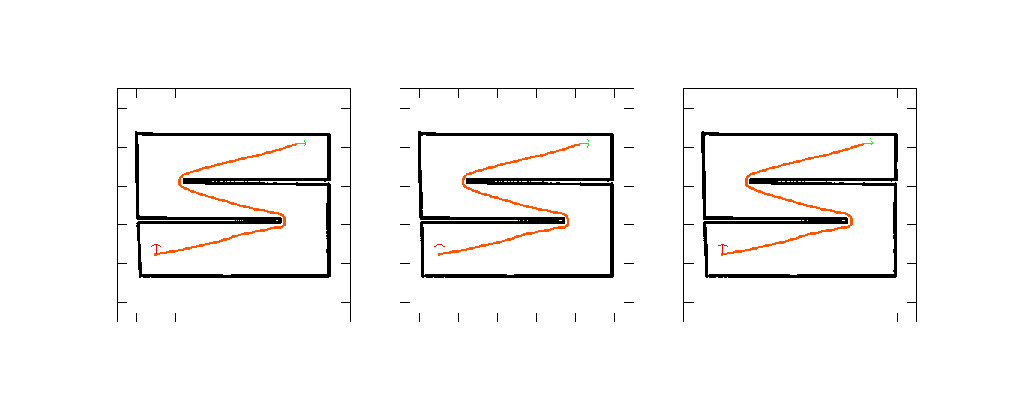
\includegraphics{./figures/parts/02/chapters/01/sections/04/global_plan_navfn_corridor}}%
    \gplfronttext
  \end{picture}%
\endgroup

  \end{subfigure}\\%
  \vspace{-1cm}
  \begin{subfigure}[t]{\linewidth}
    \centering
    % GNUPLOT: LaTeX picture with Postscript
\begingroup
  \makeatletter
  \providecommand\color[2][]{%
    \GenericError{(gnuplot) \space\space\space\@spaces}{%
      Package color not loaded in conjunction with
      terminal option `colourtext'%
    }{See the gnuplot documentation for explanation.%
    }{Either use 'blacktext' in gnuplot or load the package
      color.sty in LaTeX.}%
    \renewcommand\color[2][]{}%
  }%
  \providecommand\includegraphics[2][]{%
    \GenericError{(gnuplot) \space\space\space\@spaces}{%
      Package graphicx or graphics not loaded%
    }{See the gnuplot documentation for explanation.%
    }{The gnuplot epslatex terminal needs graphicx.sty or graphics.sty.}%
    \renewcommand\includegraphics[2][]{}%
  }%
  \providecommand\rotatebox[2]{#2}%
  \@ifundefined{ifGPcolor}{%
    \newif\ifGPcolor
    \GPcolorfalse
  }{}%
  \@ifundefined{ifGPblacktext}{%
    \newif\ifGPblacktext
    \GPblacktexttrue
  }{}%
  % define a \g@addto@macro without @ in the name:
  \let\gplgaddtomacro\g@addto@macro
  % define empty templates for all commands taking text:
  \gdef\gplfronttext{}%
  \gdef\gplfronttext{}%
  \makeatother
  \ifGPblacktext
    % no textcolor at all
    \def\colorrgb#1{}%
    \def\colorgray#1{}%
  \else
    % gray or color?
    \ifGPcolor
      \def\colorrgb#1{\color[rgb]{#1}}%
      \def\colorgray#1{\color[gray]{#1}}%
      \expandafter\def\csname LTw\endcsname{\color{white}}%
      \expandafter\def\csname LTb\endcsname{\color{black}}%
      \expandafter\def\csname LTa\endcsname{\color{black}}%
      \expandafter\def\csname LT0\endcsname{\color[rgb]{1,0,0}}%
      \expandafter\def\csname LT1\endcsname{\color[rgb]{0,1,0}}%
      \expandafter\def\csname LT2\endcsname{\color[rgb]{0,0,1}}%
      \expandafter\def\csname LT3\endcsname{\color[rgb]{1,0,1}}%
      \expandafter\def\csname LT4\endcsname{\color[rgb]{0,1,1}}%
      \expandafter\def\csname LT5\endcsname{\color[rgb]{1,1,0}}%
      \expandafter\def\csname LT6\endcsname{\color[rgb]{0,0,0}}%
      \expandafter\def\csname LT7\endcsname{\color[rgb]{1,0.3,0}}%
      \expandafter\def\csname LT8\endcsname{\color[rgb]{0.5,0.5,0.5}}%
    \else
      % gray
      \def\colorrgb#1{\color{black}}%
      \def\colorgray#1{\color[gray]{#1}}%
      \expandafter\def\csname LTw\endcsname{\color{white}}%
      \expandafter\def\csname LTb\endcsname{\color{black}}%
      \expandafter\def\csname LTa\endcsname{\color{black}}%
      \expandafter\def\csname LT0\endcsname{\color{black}}%
      \expandafter\def\csname LT1\endcsname{\color{black}}%
      \expandafter\def\csname LT2\endcsname{\color{black}}%
      \expandafter\def\csname LT3\endcsname{\color{black}}%
      \expandafter\def\csname LT4\endcsname{\color{black}}%
      \expandafter\def\csname LT5\endcsname{\color{black}}%
      \expandafter\def\csname LT6\endcsname{\color{black}}%
      \expandafter\def\csname LT7\endcsname{\color{black}}%
      \expandafter\def\csname LT8\endcsname{\color{black}}%
    \fi
  \fi
  \setlength{\unitlength}{0.0500bp}%
  \begin{picture}(9600.00,3600.00)%
    \gplgaddtomacro\gplfronttext{%
      \colorrgb{0.00,0.00,0.00}%
      \put(828,867){\makebox(0,0)[r]{\strut{}$4$}}%
      \colorrgb{0.00,0.00,0.00}%
      \put(828,1240){\makebox(0,0)[r]{\strut{}$6$}}%
      \colorrgb{0.00,0.00,0.00}%
      \put(828,1613){\makebox(0,0)[r]{\strut{}$8$}}%
      \colorrgb{0.00,0.00,0.00}%
      \put(828,1986){\makebox(0,0)[r]{\strut{}$10$}}%
      \colorrgb{0.00,0.00,0.00}%
      \put(828,2359){\makebox(0,0)[r]{\strut{}$12$}}%
      \colorrgb{0.00,0.00,0.00}%
      \put(828,2732){\makebox(0,0)[r]{\strut{}$14$}}%
      \put(322,1799){\rotatebox{90}{\makebox(0,0){\strut{}$y$ [m]}}}%
      \colorrgb{0.00,0.00,0.00}%
      \put(2079,3249){\makebox(0,0){\strut{}\texttt{global\_planner} / \texttt{dwa}}}%
    }%
    \gplgaddtomacro\gplfronttext{%
    }%
    \gplgaddtomacro\gplfronttext{%
      \put(4799,3249){\makebox(0,0){\strut{}\texttt{global\_planner} / \texttt{eband}}}%
    }%
    \gplgaddtomacro\gplfronttext{%
    }%
    \gplgaddtomacro\gplfronttext{%
      \put(7519,3249){\makebox(0,0){\strut{}\texttt{global\_planner} / \texttt{teb}}}%
    }%
    \gplgaddtomacro\gplfronttext{%
    }%
    \put(0,0){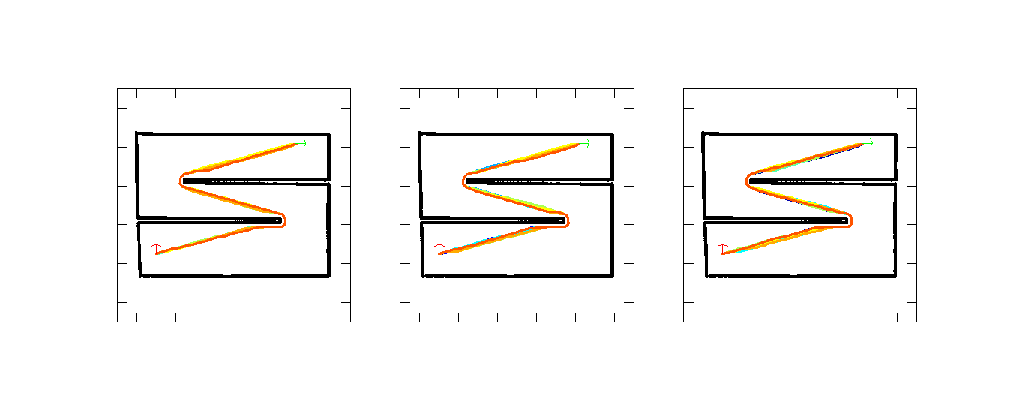
\includegraphics{./figures/parts/02/chapters/01/sections/04/global_plan_globalplanner_corridor}}%
    \gplfronttext
  \end{picture}%
\endgroup

  \end{subfigure}\\%
  \vspace{-1cm}
  \begin{subfigure}[t]{\linewidth}
    \centering
    % GNUPLOT: LaTeX picture with Postscript
\begingroup
  \makeatletter
  \providecommand\color[2][]{%
    \GenericError{(gnuplot) \space\space\space\@spaces}{%
      Package color not loaded in conjunction with
      terminal option `colourtext'%
    }{See the gnuplot documentation for explanation.%
    }{Either use 'blacktext' in gnuplot or load the package
      color.sty in LaTeX.}%
    \renewcommand\color[2][]{}%
  }%
  \providecommand\includegraphics[2][]{%
    \GenericError{(gnuplot) \space\space\space\@spaces}{%
      Package graphicx or graphics not loaded%
    }{See the gnuplot documentation for explanation.%
    }{The gnuplot epslatex terminal needs graphicx.sty or graphics.sty.}%
    \renewcommand\includegraphics[2][]{}%
  }%
  \providecommand\rotatebox[2]{#2}%
  \@ifundefined{ifGPcolor}{%
    \newif\ifGPcolor
    \GPcolorfalse
  }{}%
  \@ifundefined{ifGPblacktext}{%
    \newif\ifGPblacktext
    \GPblacktexttrue
  }{}%
  % define a \g@addto@macro without @ in the name:
  \let\gplgaddtomacro\g@addto@macro
  % define empty templates for all commands taking text:
  \gdef\gplfronttext{}%
  \gdef\gplfronttext{}%
  \makeatother
  \ifGPblacktext
    % no textcolor at all
    \def\colorrgb#1{}%
    \def\colorgray#1{}%
  \else
    % gray or color?
    \ifGPcolor
      \def\colorrgb#1{\color[rgb]{#1}}%
      \def\colorgray#1{\color[gray]{#1}}%
      \expandafter\def\csname LTw\endcsname{\color{white}}%
      \expandafter\def\csname LTb\endcsname{\color{black}}%
      \expandafter\def\csname LTa\endcsname{\color{black}}%
      \expandafter\def\csname LT0\endcsname{\color[rgb]{1,0,0}}%
      \expandafter\def\csname LT1\endcsname{\color[rgb]{0,1,0}}%
      \expandafter\def\csname LT2\endcsname{\color[rgb]{0,0,1}}%
      \expandafter\def\csname LT3\endcsname{\color[rgb]{1,0,1}}%
      \expandafter\def\csname LT4\endcsname{\color[rgb]{0,1,1}}%
      \expandafter\def\csname LT5\endcsname{\color[rgb]{1,1,0}}%
      \expandafter\def\csname LT6\endcsname{\color[rgb]{0,0,0}}%
      \expandafter\def\csname LT7\endcsname{\color[rgb]{1,0.3,0}}%
      \expandafter\def\csname LT8\endcsname{\color[rgb]{0.5,0.5,0.5}}%
    \else
      % gray
      \def\colorrgb#1{\color{black}}%
      \def\colorgray#1{\color[gray]{#1}}%
      \expandafter\def\csname LTw\endcsname{\color{white}}%
      \expandafter\def\csname LTb\endcsname{\color{black}}%
      \expandafter\def\csname LTa\endcsname{\color{black}}%
      \expandafter\def\csname LT0\endcsname{\color{black}}%
      \expandafter\def\csname LT1\endcsname{\color{black}}%
      \expandafter\def\csname LT2\endcsname{\color{black}}%
      \expandafter\def\csname LT3\endcsname{\color{black}}%
      \expandafter\def\csname LT4\endcsname{\color{black}}%
      \expandafter\def\csname LT5\endcsname{\color{black}}%
      \expandafter\def\csname LT6\endcsname{\color{black}}%
      \expandafter\def\csname LT7\endcsname{\color{black}}%
      \expandafter\def\csname LT8\endcsname{\color{black}}%
    \fi
  \fi
  \setlength{\unitlength}{0.0500bp}%
  \begin{picture}(9600.00,3600.00)%
    \gplgaddtomacro\gplfronttext{%
      \colorrgb{0.00,0.00,0.00}%
      \put(828,867){\makebox(0,0)[r]{\strut{}$4$}}%
      \colorrgb{0.00,0.00,0.00}%
      \put(828,1240){\makebox(0,0)[r]{\strut{}$6$}}%
      \colorrgb{0.00,0.00,0.00}%
      \put(828,1613){\makebox(0,0)[r]{\strut{}$8$}}%
      \colorrgb{0.00,0.00,0.00}%
      \put(828,1986){\makebox(0,0)[r]{\strut{}$10$}}%
      \colorrgb{0.00,0.00,0.00}%
      \put(828,2359){\makebox(0,0)[r]{\strut{}$12$}}%
      \colorrgb{0.00,0.00,0.00}%
      \put(828,2732){\makebox(0,0)[r]{\strut{}$14$}}%
      \colorrgb{0.00,0.00,0.00}%
      \put(1147,460){\makebox(0,0){\strut{}$4$}}%
      \colorrgb{0.00,0.00,0.00}%
      \put(1520,460){\makebox(0,0){\strut{}$6$}}%
      \colorrgb{0.00,0.00,0.00}%
      \put(1893,460){\makebox(0,0){\strut{}$8$}}%
      \colorrgb{0.00,0.00,0.00}%
      \put(2266,460){\makebox(0,0){\strut{}$10$}}%
      \colorrgb{0.00,0.00,0.00}%
      \put(2639,460){\makebox(0,0){\strut{}$12$}}%
      \colorrgb{0.00,0.00,0.00}%
      \put(3012,460){\makebox(0,0){\strut{}$14$}}%
      \colorrgb{0.00,0.00,0.00}%
      \put(322,1799){\rotatebox{90}{\makebox(0,0){\strut{}$y$ [m]}}}%
      \colorrgb{0.00,0.00,0.00}%
      \put(2079,130){\makebox(0,0){\strut{}$x$ [m]}}%
      \colorrgb{0.00,0.00,0.00}%
      \put(2079,3199){\makebox(0,0){\strut{}\texttt{sbpl} / \texttt{dwa}}}%
    }%
    \gplgaddtomacro\gplfronttext{%
    }%
    \gplgaddtomacro\gplfronttext{%
      \colorrgb{0.00,0.00,0.00}%
      \put(3866,460){\makebox(0,0){\strut{}$4$}}%
      \colorrgb{0.00,0.00,0.00}%
      \put(4239,460){\makebox(0,0){\strut{}$6$}}%
      \colorrgb{0.00,0.00,0.00}%
      \put(4612,460){\makebox(0,0){\strut{}$8$}}%
      \colorrgb{0.00,0.00,0.00}%
      \put(4986,460){\makebox(0,0){\strut{}$10$}}%
      \colorrgb{0.00,0.00,0.00}%
      \put(5359,460){\makebox(0,0){\strut{}$12$}}%
      \colorrgb{0.00,0.00,0.00}%
      \put(5732,460){\makebox(0,0){\strut{}$14$}}%
      \colorrgb{0.00,0.00,0.00}%
      \put(4799,130){\makebox(0,0){\strut{}$x$ [m]}}%
      \colorrgb{0.00,0.00,0.00}%
      \put(4799,3199){\makebox(0,0){\strut{}\texttt{sbpl} / \texttt{eband}}}%
    }%
    \gplgaddtomacro\gplfronttext{%
    }%
    \gplgaddtomacro\gplfronttext{%
      \colorrgb{0.00,0.00,0.00}%
      \put(6587,460){\makebox(0,0){\strut{}$4$}}%
      \colorrgb{0.00,0.00,0.00}%
      \put(6960,460){\makebox(0,0){\strut{}$6$}}%
      \colorrgb{0.00,0.00,0.00}%
      \put(7333,460){\makebox(0,0){\strut{}$8$}}%
      \colorrgb{0.00,0.00,0.00}%
      \put(7706,460){\makebox(0,0){\strut{}$10$}}%
      \colorrgb{0.00,0.00,0.00}%
      \put(8079,460){\makebox(0,0){\strut{}$12$}}%
      \colorrgb{0.00,0.00,0.00}%
      \put(8452,460){\makebox(0,0){\strut{}$14$}}%
      \colorrgb{0.00,0.00,0.00}%
      \put(7519,130){\makebox(0,0){\strut{}$x$ [m]}}%
      \colorrgb{0.00,0.00,0.00}%
      \put(7519,3199){\makebox(0,0){\strut{}\texttt{sbpl} / \texttt{teb}}}%
    }%
    \gplgaddtomacro\gplfronttext{%
    }%
    \put(0,0){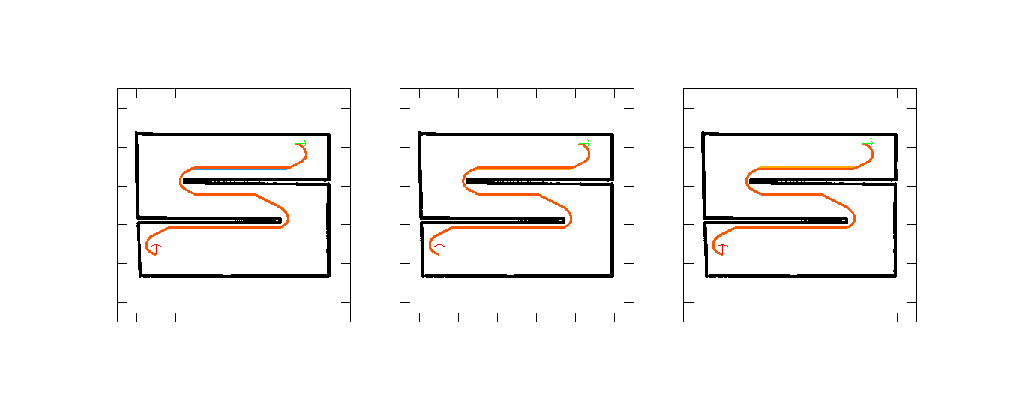
\includegraphics{./figures/parts/02/chapters/01/sections/04/global_plan_sbpl_corridor}}%
    \gplfronttext
  \end{picture}%
\endgroup

  \end{subfigure}%
  \caption{\small Τα σχεδιασθέντα μονοπάτια προς ακολούθηση $\bm{\mathcal{G}}$
           που παρήχθησαν από τους τρεις αλγορίθμους χάραξης μονοπατιών για
           κάθε συνδυασμό τους με ελεγκτή κίνησης του πίνακα
           \ref{tbl:planners_sifted_list}, σε σχέση με τις ορισμένες αρχικές και
           τελικές στάσεις του περιβάλλοντος CORRIDOR}
  \label{fig:global_plans:corridor}
\end{figure}

Το σχήμα \ref{fig:ground_truths:corridor} απεικονίζει τις πραγματικές διαδρομές
που διένυσε το ρομπότ για όλους τους συνδυασμούς αλγορίθμων σχεδίασης μονοπατιών
και ελεγκτών κίνησης του ίδιου πίνακα, για $N=10$ προσομοιώσεις για κάθε
συνδυασμό.

\begin{figure}\centering
  \begin{subfigure}[t]{\linewidth}
    \centering
    % GNUPLOT: LaTeX picture with Postscript
\begingroup
  \makeatletter
  \providecommand\color[2][]{%
    \GenericError{(gnuplot) \space\space\space\@spaces}{%
      Package color not loaded in conjunction with
      terminal option `colourtext'%
    }{See the gnuplot documentation for explanation.%
    }{Either use 'blacktext' in gnuplot or load the package
      color.sty in LaTeX.}%
    \renewcommand\color[2][]{}%
  }%
  \providecommand\includegraphics[2][]{%
    \GenericError{(gnuplot) \space\space\space\@spaces}{%
      Package graphicx or graphics not loaded%
    }{See the gnuplot documentation for explanation.%
    }{The gnuplot epslatex terminal needs graphicx.sty or graphics.sty.}%
    \renewcommand\includegraphics[2][]{}%
  }%
  \providecommand\rotatebox[2]{#2}%
  \@ifundefined{ifGPcolor}{%
    \newif\ifGPcolor
    \GPcolorfalse
  }{}%
  \@ifundefined{ifGPblacktext}{%
    \newif\ifGPblacktext
    \GPblacktexttrue
  }{}%
  % define a \g@addto@macro without @ in the name:
  \let\gplgaddtomacro\g@addto@macro
  % define empty templates for all commands taking text:
  \gdef\gplfronttext{}%
  \gdef\gplfronttext{}%
  \makeatother
  \ifGPblacktext
    % no textcolor at all
    \def\colorrgb#1{}%
    \def\colorgray#1{}%
  \else
    % gray or color?
    \ifGPcolor
      \def\colorrgb#1{\color[rgb]{#1}}%
      \def\colorgray#1{\color[gray]{#1}}%
      \expandafter\def\csname LTw\endcsname{\color{white}}%
      \expandafter\def\csname LTb\endcsname{\color{black}}%
      \expandafter\def\csname LTa\endcsname{\color{black}}%
      \expandafter\def\csname LT0\endcsname{\color[rgb]{1,0,0}}%
      \expandafter\def\csname LT1\endcsname{\color[rgb]{0,1,0}}%
      \expandafter\def\csname LT2\endcsname{\color[rgb]{0,0,1}}%
      \expandafter\def\csname LT3\endcsname{\color[rgb]{1,0,1}}%
      \expandafter\def\csname LT4\endcsname{\color[rgb]{0,1,1}}%
      \expandafter\def\csname LT5\endcsname{\color[rgb]{1,1,0}}%
      \expandafter\def\csname LT6\endcsname{\color[rgb]{0,0,0}}%
      \expandafter\def\csname LT7\endcsname{\color[rgb]{1,0.3,0}}%
      \expandafter\def\csname LT8\endcsname{\color[rgb]{0.5,0.5,0.5}}%
    \else
      % gray
      \def\colorrgb#1{\color{black}}%
      \def\colorgray#1{\color[gray]{#1}}%
      \expandafter\def\csname LTw\endcsname{\color{white}}%
      \expandafter\def\csname LTb\endcsname{\color{black}}%
      \expandafter\def\csname LTa\endcsname{\color{black}}%
      \expandafter\def\csname LT0\endcsname{\color{black}}%
      \expandafter\def\csname LT1\endcsname{\color{black}}%
      \expandafter\def\csname LT2\endcsname{\color{black}}%
      \expandafter\def\csname LT3\endcsname{\color{black}}%
      \expandafter\def\csname LT4\endcsname{\color{black}}%
      \expandafter\def\csname LT5\endcsname{\color{black}}%
      \expandafter\def\csname LT6\endcsname{\color{black}}%
      \expandafter\def\csname LT7\endcsname{\color{black}}%
      \expandafter\def\csname LT8\endcsname{\color{black}}%
    \fi
  \fi
  \setlength{\unitlength}{0.0500bp}%
  \begin{picture}(9600.00,3600.00)%
    \gplgaddtomacro\gplfronttext{%
      \colorrgb{0.00,0.00,0.00}%
      \put(828,867){\makebox(0,0)[r]{\strut{}$4$}}%
      \colorrgb{0.00,0.00,0.00}%
      \put(828,1240){\makebox(0,0)[r]{\strut{}$6$}}%
      \colorrgb{0.00,0.00,0.00}%
      \put(828,1613){\makebox(0,0)[r]{\strut{}$8$}}%
      \colorrgb{0.00,0.00,0.00}%
      \put(828,1986){\makebox(0,0)[r]{\strut{}$10$}}%
      \colorrgb{0.00,0.00,0.00}%
      \put(828,2359){\makebox(0,0)[r]{\strut{}$12$}}%
      \colorrgb{0.00,0.00,0.00}%
      \put(828,2732){\makebox(0,0)[r]{\strut{}$14$}}%
      \put(322,1799){\rotatebox{90}{\makebox(0,0){\strut{}$y$ [m]}}}%
      \colorrgb{0.00,0.00,0.00}%
      \put(2079,3199){\makebox(0,0){\strut{}\texttt{navfn} / \texttt{dwa}}}%
    }%
    \gplgaddtomacro\gplfronttext{%
    }%
    \gplgaddtomacro\gplfronttext{%
      \put(4799,3199){\makebox(0,0){\strut{}\texttt{navfn} / \texttt{eband}}}%
    }%
    \gplgaddtomacro\gplfronttext{%
    }%
    \gplgaddtomacro\gplfronttext{%
      \put(7519,3199){\makebox(0,0){\strut{}\texttt{navfn} / \texttt{teb}}}%
    }%
    \gplgaddtomacro\gplfronttext{%
    }%
    \put(0,0){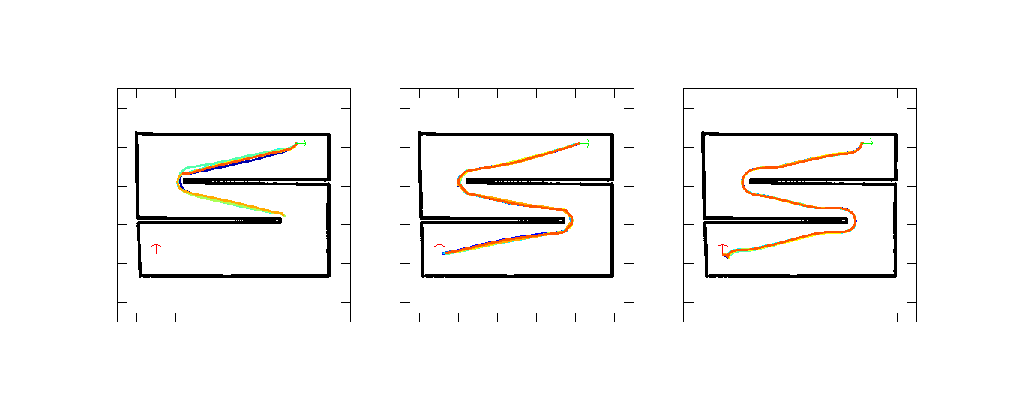
\includegraphics{./figures/parts/02/chapters/01/sections/04/ground_truth_navfn_corridor}}%
    \gplfronttext
  \end{picture}%
\endgroup

  \end{subfigure}\\%
  \vspace{-1cm}
  \begin{subfigure}[t]{\linewidth}
    \centering
    % GNUPLOT: LaTeX picture with Postscript
\begingroup
  \makeatletter
  \providecommand\color[2][]{%
    \GenericError{(gnuplot) \space\space\space\@spaces}{%
      Package color not loaded in conjunction with
      terminal option `colourtext'%
    }{See the gnuplot documentation for explanation.%
    }{Either use 'blacktext' in gnuplot or load the package
      color.sty in LaTeX.}%
    \renewcommand\color[2][]{}%
  }%
  \providecommand\includegraphics[2][]{%
    \GenericError{(gnuplot) \space\space\space\@spaces}{%
      Package graphicx or graphics not loaded%
    }{See the gnuplot documentation for explanation.%
    }{The gnuplot epslatex terminal needs graphicx.sty or graphics.sty.}%
    \renewcommand\includegraphics[2][]{}%
  }%
  \providecommand\rotatebox[2]{#2}%
  \@ifundefined{ifGPcolor}{%
    \newif\ifGPcolor
    \GPcolorfalse
  }{}%
  \@ifundefined{ifGPblacktext}{%
    \newif\ifGPblacktext
    \GPblacktexttrue
  }{}%
  % define a \g@addto@macro without @ in the name:
  \let\gplgaddtomacro\g@addto@macro
  % define empty templates for all commands taking text:
  \gdef\gplfronttext{}%
  \gdef\gplfronttext{}%
  \makeatother
  \ifGPblacktext
    % no textcolor at all
    \def\colorrgb#1{}%
    \def\colorgray#1{}%
  \else
    % gray or color?
    \ifGPcolor
      \def\colorrgb#1{\color[rgb]{#1}}%
      \def\colorgray#1{\color[gray]{#1}}%
      \expandafter\def\csname LTw\endcsname{\color{white}}%
      \expandafter\def\csname LTb\endcsname{\color{black}}%
      \expandafter\def\csname LTa\endcsname{\color{black}}%
      \expandafter\def\csname LT0\endcsname{\color[rgb]{1,0,0}}%
      \expandafter\def\csname LT1\endcsname{\color[rgb]{0,1,0}}%
      \expandafter\def\csname LT2\endcsname{\color[rgb]{0,0,1}}%
      \expandafter\def\csname LT3\endcsname{\color[rgb]{1,0,1}}%
      \expandafter\def\csname LT4\endcsname{\color[rgb]{0,1,1}}%
      \expandafter\def\csname LT5\endcsname{\color[rgb]{1,1,0}}%
      \expandafter\def\csname LT6\endcsname{\color[rgb]{0,0,0}}%
      \expandafter\def\csname LT7\endcsname{\color[rgb]{1,0.3,0}}%
      \expandafter\def\csname LT8\endcsname{\color[rgb]{0.5,0.5,0.5}}%
    \else
      % gray
      \def\colorrgb#1{\color{black}}%
      \def\colorgray#1{\color[gray]{#1}}%
      \expandafter\def\csname LTw\endcsname{\color{white}}%
      \expandafter\def\csname LTb\endcsname{\color{black}}%
      \expandafter\def\csname LTa\endcsname{\color{black}}%
      \expandafter\def\csname LT0\endcsname{\color{black}}%
      \expandafter\def\csname LT1\endcsname{\color{black}}%
      \expandafter\def\csname LT2\endcsname{\color{black}}%
      \expandafter\def\csname LT3\endcsname{\color{black}}%
      \expandafter\def\csname LT4\endcsname{\color{black}}%
      \expandafter\def\csname LT5\endcsname{\color{black}}%
      \expandafter\def\csname LT6\endcsname{\color{black}}%
      \expandafter\def\csname LT7\endcsname{\color{black}}%
      \expandafter\def\csname LT8\endcsname{\color{black}}%
    \fi
  \fi
  \setlength{\unitlength}{0.0500bp}%
  \begin{picture}(9600.00,3600.00)%
    \gplgaddtomacro\gplfronttext{%
      \colorrgb{0.00,0.00,0.00}%
      \put(828,867){\makebox(0,0)[r]{\strut{}$4$}}%
      \colorrgb{0.00,0.00,0.00}%
      \put(828,1240){\makebox(0,0)[r]{\strut{}$6$}}%
      \colorrgb{0.00,0.00,0.00}%
      \put(828,1613){\makebox(0,0)[r]{\strut{}$8$}}%
      \colorrgb{0.00,0.00,0.00}%
      \put(828,1986){\makebox(0,0)[r]{\strut{}$10$}}%
      \colorrgb{0.00,0.00,0.00}%
      \put(828,2359){\makebox(0,0)[r]{\strut{}$12$}}%
      \colorrgb{0.00,0.00,0.00}%
      \put(828,2732){\makebox(0,0)[r]{\strut{}$14$}}%
      \put(322,1799){\rotatebox{90}{\makebox(0,0){\strut{}$y$ [m]}}}%
      \colorrgb{0.00,0.00,0.00}%
      \put(2079,3199){\makebox(0,0){\strut{}\texttt{global\_planner} / \texttt{dwa}}}%
    }%
    \gplgaddtomacro\gplfronttext{%
    }%
    \gplgaddtomacro\gplfronttext{%
      \put(4799,3199){\makebox(0,0){\strut{}\texttt{global\_planner} / \texttt{eband}}}%
    }%
    \gplgaddtomacro\gplfronttext{%
    }%
    \gplgaddtomacro\gplfronttext{%
      \put(7519,3199){\makebox(0,0){\strut{}\texttt{global\_planner} / \texttt{teb}}}%
    }%
    \gplgaddtomacro\gplfronttext{%
    }%
    \put(0,0){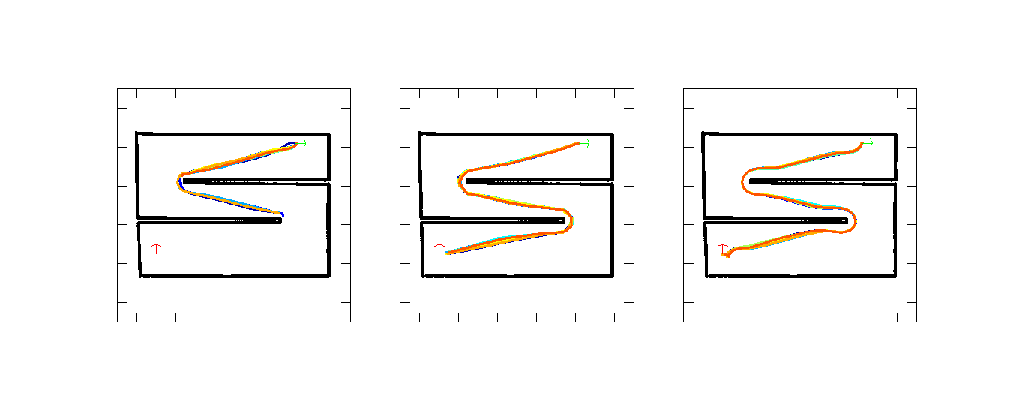
\includegraphics{./figures/parts/02/chapters/01/sections/04/ground_truth_globalplanner_corridor}}%
    \gplfronttext
  \end{picture}%
\endgroup

  \end{subfigure}\\%
  \vspace{-1cm}
  \begin{subfigure}[t]{\linewidth}
    \centering
    % GNUPLOT: LaTeX picture with Postscript
\begingroup
  \makeatletter
  \providecommand\color[2][]{%
    \GenericError{(gnuplot) \space\space\space\@spaces}{%
      Package color not loaded in conjunction with
      terminal option `colourtext'%
    }{See the gnuplot documentation for explanation.%
    }{Either use 'blacktext' in gnuplot or load the package
      color.sty in LaTeX.}%
    \renewcommand\color[2][]{}%
  }%
  \providecommand\includegraphics[2][]{%
    \GenericError{(gnuplot) \space\space\space\@spaces}{%
      Package graphicx or graphics not loaded%
    }{See the gnuplot documentation for explanation.%
    }{The gnuplot epslatex terminal needs graphicx.sty or graphics.sty.}%
    \renewcommand\includegraphics[2][]{}%
  }%
  \providecommand\rotatebox[2]{#2}%
  \@ifundefined{ifGPcolor}{%
    \newif\ifGPcolor
    \GPcolorfalse
  }{}%
  \@ifundefined{ifGPblacktext}{%
    \newif\ifGPblacktext
    \GPblacktexttrue
  }{}%
  % define a \g@addto@macro without @ in the name:
  \let\gplgaddtomacro\g@addto@macro
  % define empty templates for all commands taking text:
  \gdef\gplfronttext{}%
  \gdef\gplfronttext{}%
  \makeatother
  \ifGPblacktext
    % no textcolor at all
    \def\colorrgb#1{}%
    \def\colorgray#1{}%
  \else
    % gray or color?
    \ifGPcolor
      \def\colorrgb#1{\color[rgb]{#1}}%
      \def\colorgray#1{\color[gray]{#1}}%
      \expandafter\def\csname LTw\endcsname{\color{white}}%
      \expandafter\def\csname LTb\endcsname{\color{black}}%
      \expandafter\def\csname LTa\endcsname{\color{black}}%
      \expandafter\def\csname LT0\endcsname{\color[rgb]{1,0,0}}%
      \expandafter\def\csname LT1\endcsname{\color[rgb]{0,1,0}}%
      \expandafter\def\csname LT2\endcsname{\color[rgb]{0,0,1}}%
      \expandafter\def\csname LT3\endcsname{\color[rgb]{1,0,1}}%
      \expandafter\def\csname LT4\endcsname{\color[rgb]{0,1,1}}%
      \expandafter\def\csname LT5\endcsname{\color[rgb]{1,1,0}}%
      \expandafter\def\csname LT6\endcsname{\color[rgb]{0,0,0}}%
      \expandafter\def\csname LT7\endcsname{\color[rgb]{1,0.3,0}}%
      \expandafter\def\csname LT8\endcsname{\color[rgb]{0.5,0.5,0.5}}%
    \else
      % gray
      \def\colorrgb#1{\color{black}}%
      \def\colorgray#1{\color[gray]{#1}}%
      \expandafter\def\csname LTw\endcsname{\color{white}}%
      \expandafter\def\csname LTb\endcsname{\color{black}}%
      \expandafter\def\csname LTa\endcsname{\color{black}}%
      \expandafter\def\csname LT0\endcsname{\color{black}}%
      \expandafter\def\csname LT1\endcsname{\color{black}}%
      \expandafter\def\csname LT2\endcsname{\color{black}}%
      \expandafter\def\csname LT3\endcsname{\color{black}}%
      \expandafter\def\csname LT4\endcsname{\color{black}}%
      \expandafter\def\csname LT5\endcsname{\color{black}}%
      \expandafter\def\csname LT6\endcsname{\color{black}}%
      \expandafter\def\csname LT7\endcsname{\color{black}}%
      \expandafter\def\csname LT8\endcsname{\color{black}}%
    \fi
  \fi
  \setlength{\unitlength}{0.0500bp}%
  \begin{picture}(9600.00,3600.00)%
    \gplgaddtomacro\gplfronttext{%
      \colorrgb{0.00,0.00,0.00}%
      \put(828,867){\makebox(0,0)[r]{\strut{}$4$}}%
      \colorrgb{0.00,0.00,0.00}%
      \put(828,1240){\makebox(0,0)[r]{\strut{}$6$}}%
      \colorrgb{0.00,0.00,0.00}%
      \put(828,1613){\makebox(0,0)[r]{\strut{}$8$}}%
      \colorrgb{0.00,0.00,0.00}%
      \put(828,1986){\makebox(0,0)[r]{\strut{}$10$}}%
      \colorrgb{0.00,0.00,0.00}%
      \put(828,2359){\makebox(0,0)[r]{\strut{}$12$}}%
      \colorrgb{0.00,0.00,0.00}%
      \put(828,2732){\makebox(0,0)[r]{\strut{}$14$}}%
      \colorrgb{0.00,0.00,0.00}%
      \put(1147,460){\makebox(0,0){\strut{}$4$}}%
      \colorrgb{0.00,0.00,0.00}%
      \put(1520,460){\makebox(0,0){\strut{}$6$}}%
      \colorrgb{0.00,0.00,0.00}%
      \put(1893,460){\makebox(0,0){\strut{}$8$}}%
      \colorrgb{0.00,0.00,0.00}%
      \put(2266,460){\makebox(0,0){\strut{}$10$}}%
      \colorrgb{0.00,0.00,0.00}%
      \put(2639,460){\makebox(0,0){\strut{}$12$}}%
      \colorrgb{0.00,0.00,0.00}%
      \put(3012,460){\makebox(0,0){\strut{}$14$}}%
      \colorrgb{0.00,0.00,0.00}%
      \put(322,1799){\rotatebox{90}{\makebox(0,0){\strut{}$y$ [m]}}}%
      \colorrgb{0.00,0.00,0.00}%
      \put(2079,130){\makebox(0,0){\strut{}$x$ [m]}}%
      \colorrgb{0.00,0.00,0.00}%
      \put(2079,3199){\makebox(0,0){\strut{}\texttt{sbpl} / \texttt{dwa}}}%
    }%
    \gplgaddtomacro\gplfronttext{%
    }%
    \gplgaddtomacro\gplfronttext{%
      \put(3866,460){\makebox(0,0){\strut{}$4$}}%
      \colorrgb{0.00,0.00,0.00}%
      \put(4239,460){\makebox(0,0){\strut{}$6$}}%
      \colorrgb{0.00,0.00,0.00}%
      \put(4612,460){\makebox(0,0){\strut{}$8$}}%
      \colorrgb{0.00,0.00,0.00}%
      \put(4986,460){\makebox(0,0){\strut{}$10$}}%
      \colorrgb{0.00,0.00,0.00}%
      \put(5359,460){\makebox(0,0){\strut{}$12$}}%
      \colorrgb{0.00,0.00,0.00}%
      \put(5732,460){\makebox(0,0){\strut{}$14$}}%
      \colorrgb{0.00,0.00,0.00}%
      \put(4799,130){\makebox(0,0){\strut{}$x$ [m]}}%
      \colorrgb{0.00,0.00,0.00}%
      \put(4799,3199){\makebox(0,0){\strut{}\texttt{sbpl} / \texttt{eband}}}%
    }%
    \gplgaddtomacro\gplfronttext{%
    }%
    \gplgaddtomacro\gplfronttext{%
      \put(6587,460){\makebox(0,0){\strut{}$4$}}%
      \colorrgb{0.00,0.00,0.00}%
      \put(6960,460){\makebox(0,0){\strut{}$6$}}%
      \colorrgb{0.00,0.00,0.00}%
      \put(7333,460){\makebox(0,0){\strut{}$8$}}%
      \colorrgb{0.00,0.00,0.00}%
      \put(7706,460){\makebox(0,0){\strut{}$10$}}%
      \colorrgb{0.00,0.00,0.00}%
      \put(8079,460){\makebox(0,0){\strut{}$12$}}%
      \colorrgb{0.00,0.00,0.00}%
      \put(8452,460){\makebox(0,0){\strut{}$14$}}%
      \colorrgb{0.00,0.00,0.00}%
      \put(7519,130){\makebox(0,0){\strut{}$x$ [m]}}%
      \colorrgb{0.00,0.00,0.00}%
      \put(7519,3199){\makebox(0,0){\strut{}\texttt{sbpl} / \texttt{teb}}}%
    }%
    \gplgaddtomacro\gplfronttext{%
    }%
    \put(0,0){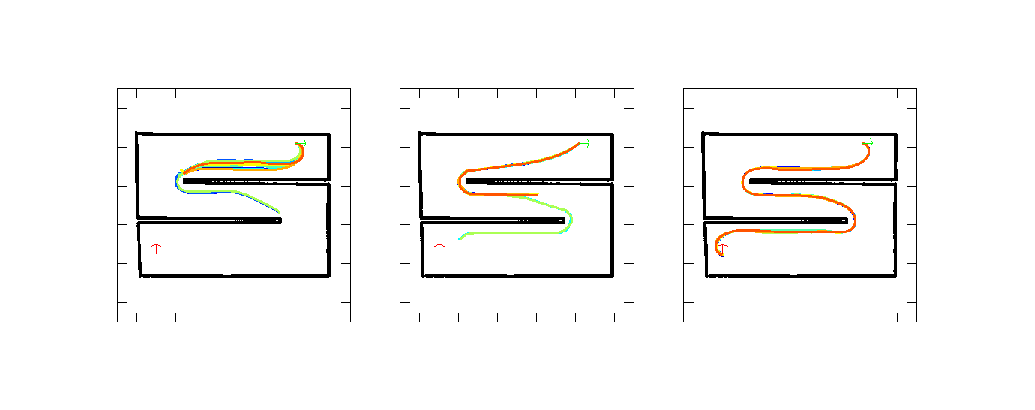
\includegraphics{./figures/parts/02/chapters/01/sections/04/ground_truth_sbpl_corridor}}%
    \gplfronttext
  \end{picture}%
\endgroup

  \end{subfigure}%
  \caption{\small Τα διανυθέντα μονοπάτια $\bm{\mathcal{P}}$ του ρομπότ, όπως
           ορίστηκαν από τους τρεις ελεγκτές κίνησης για κάθε συνδυασμό τους με
           αλγόριθμο παραγωγής μονοπατιών του πίνακα
           \ref{tbl:planners_sifted_list}, σε σχέση με τις ορισμένες αρχικές και
           τελικές στάσεις του περιβάλλοντος CORRIDOR}
  \label{fig:ground_truths:corridor}
\end{figure}


Ο πίνακας \ref{tbl:rank_corridor} καταγράφει την τιμή-αξία $V_{\bm{M}_C}$ και
την κατάταξη όλων των συνδυασμών αλγορίθμων χάραξης μονοπατιών και ελεγκτών
κίνησης που αξιολογήθηκαν με βάση τις τιμές όλων των μετρικών, που
παρουσιάζονται στους πίνακες
\ref{tbl:info_global_plan_corridor}-\ref{tbl:info_deviation_from_global_plan_corridor},
όσον αφορά στις επιδόσεις τους στην πλοήγηση στο περιβάλλον CORRIDOR. Για τον
υπολογισμό της τιμής όλων των συνδυασμών, όλα τα βάρη $w_m = 1.0$ εκτός από
αυτό που αφορά στη μετρική $\mu_{PF} / \mu_{LPC}$, λόγω του γεγονότος ότι ότι ο
\texttt{eband\_local\_planner} δεν παρέχει πρόσβαση στον αριθμό των κλήσεων του
ελεγκτή. Συνολικά, ο ελεγκτής κίνησης \texttt{teb\_local\_planner} κατέλαβε
όλες τις θέσεις του βάθρου, με τον συνδυασμό του με τον αλγόριθμο
\texttt{navfn} να είναι ο με τις καλύτερες επιδόσεις μεταξύ των τριών.
Λεπτομέρειες σχετικά με τις επιδόσεις των αλγορίθμων χάραξης μονοπατιών, των
ελεγκτών κίνησης, και των συνδυασμών τους, βρίσκονται στο παράρτημα
\ref{appendix:evaluation_corridor}.

\begin{table}\centering
\renewcommand{\arraystretch}{1.3}
\begin{tabular}{llccc}
  GP                        & LP              & επιτυχημένες αποστολές / $N$ & $V_{\bm{M}_C}$ & Κατάταξη \\ \toprule
  \texttt{navfn}            & \texttt{teb}    & $10/10$                      & $21.41$        & $1$      \\
  \texttt{sbpl}             & \texttt{teb}    & $10/10$                      & $20.35$        & $2$      \\
  \texttt{global\_planner}  & \texttt{teb}    & $10/10$                      & $19.29$        & $3$      \\
  \texttt{navfn}            & \texttt{eband}  & $10/10$                      & $15.96$        & $4$      \\
  \texttt{global\_planner}  & \texttt{eband}  & $10/10$                      & $14.70$        & $5$      \\
  \texttt{sbpl}             & \texttt{eband}  & $0/10$                       & $10.99$        & $6$      \\
  \texttt{sbpl}             & \texttt{dwa}    & $0/10$                       & $6.56$         & $7$      \\
  \texttt{navfn}            & \texttt{dwa}    & $0/10$                       & $6.46$         & $8$      \\
  \texttt{global\_planner}  & \texttt{dwa}    & $0/10$                       & $5.50$         & $9$      \\ \bottomrule
\end{tabular}
\caption{\small Οι αριθμοί επιτυχίας αποστολών, η τιμή-αξία $V_{\bm{M}_C}$, και
         η κατάταξη όλων των συνδυασμών των αλγορίθμων χάραξης μονοπατιών και
         ελεγκτών κίνησης που αξιολογούνται για τους την επίδοσή τους στο
         περιβάλλον CORRIDOR σε $N=10$ προσομοιώσεις}
\label{tbl:rank_corridor}
\end{table}


%%%%%%%%%%%%%%%%%%%%%%%%%%%%%%%%%%%%%%%%%%%%%%%%%%%%%%%%%%%%%%%%%%%%%%%%%%%%%%%%
\subsection{Αξιολόγηση στο περιβάλλον WILLOWGARAGE}
  \label{subsection:02_01_04:03}

Συνολικά, όλοι οι συνδυασμοί των αλγόριθμο χάραξης μονοπατιών με τους
ελεγκτές κίνησης \texttt{dwa\_local\_planner} και \texttt{eband\_local\_planner}
απέτυχαν να πλοηγήσουν το ρομπότ στην τελική του στάση. Οι υπόλοιποι συνδυασμοί
(όλοι με τον \texttt{teb\_local\_planner} ως ελεγκτή κίνησής τους) ήταν
αξιόπιστοι σε κάθε προσομοίωση

Το σχήμα \ref{fig:global_plans:willowgarage} απεικονίζει τα μονοπάτια προς
ακολούθηση που παρήχθησαν από όλους τους global planners που εμφανίζονται στην
πρώτη στήλη του πίνακα \ref{tbl:planners_sifted_list}, για όλους τους
συνδυασμούς global και local planner του ίδιου πίνακα, για $N=10$ προσομοιώσεις
κάθε συνδυασμού.

\begin{figure}
\raggedright
  \begin{subfigure}[t]{\linewidth}
    \centering
    % GNUPLOT: LaTeX picture with Postscript
\begingroup
  \makeatletter
  \providecommand\color[2][]{%
    \GenericError{(gnuplot) \space\space\space\@spaces}{%
      Package color not loaded in conjunction with
      terminal option `colourtext'%
    }{See the gnuplot documentation for explanation.%
    }{Either use 'blacktext' in gnuplot or load the package
      color.sty in LaTeX.}%
    \renewcommand\color[2][]{}%
  }%
  \providecommand\includegraphics[2][]{%
    \GenericError{(gnuplot) \space\space\space\@spaces}{%
      Package graphicx or graphics not loaded%
    }{See the gnuplot documentation for explanation.%
    }{The gnuplot epslatex terminal needs graphicx.sty or graphics.sty.}%
    \renewcommand\includegraphics[2][]{}%
  }%
  \providecommand\rotatebox[2]{#2}%
  \@ifundefined{ifGPcolor}{%
    \newif\ifGPcolor
    \GPcolorfalse
  }{}%
  \@ifundefined{ifGPblacktext}{%
    \newif\ifGPblacktext
    \GPblacktexttrue
  }{}%
  % define a \g@addto@macro without @ in the name:
  \let\gplgaddtomacro\g@addto@macro
  % define empty templates for all commands taking text:
  \gdef\gplfronttext{}%
  \gdef\gplfronttext{}%
  \makeatother
  \ifGPblacktext
    % no textcolor at all
    \def\colorrgb#1{}%
    \def\colorgray#1{}%
  \else
    % gray or color?
    \ifGPcolor
      \def\colorrgb#1{\color[rgb]{#1}}%
      \def\colorgray#1{\color[gray]{#1}}%
      \expandafter\def\csname LTw\endcsname{\color{white}}%
      \expandafter\def\csname LTb\endcsname{\color{black}}%
      \expandafter\def\csname LTa\endcsname{\color{black}}%
      \expandafter\def\csname LT0\endcsname{\color[rgb]{1,0,0}}%
      \expandafter\def\csname LT1\endcsname{\color[rgb]{0,1,0}}%
      \expandafter\def\csname LT2\endcsname{\color[rgb]{0,0,1}}%
      \expandafter\def\csname LT3\endcsname{\color[rgb]{1,0,1}}%
      \expandafter\def\csname LT4\endcsname{\color[rgb]{0,1,1}}%
      \expandafter\def\csname LT5\endcsname{\color[rgb]{1,1,0}}%
      \expandafter\def\csname LT6\endcsname{\color[rgb]{0,0,0}}%
      \expandafter\def\csname LT7\endcsname{\color[rgb]{1,0.3,0}}%
      \expandafter\def\csname LT8\endcsname{\color[rgb]{0.5,0.5,0.5}}%
    \else
      % gray
      \def\colorrgb#1{\color{black}}%
      \def\colorgray#1{\color[gray]{#1}}%
      \expandafter\def\csname LTw\endcsname{\color{white}}%
      \expandafter\def\csname LTb\endcsname{\color{black}}%
      \expandafter\def\csname LTa\endcsname{\color{black}}%
      \expandafter\def\csname LT0\endcsname{\color{black}}%
      \expandafter\def\csname LT1\endcsname{\color{black}}%
      \expandafter\def\csname LT2\endcsname{\color{black}}%
      \expandafter\def\csname LT3\endcsname{\color{black}}%
      \expandafter\def\csname LT4\endcsname{\color{black}}%
      \expandafter\def\csname LT5\endcsname{\color{black}}%
      \expandafter\def\csname LT6\endcsname{\color{black}}%
      \expandafter\def\csname LT7\endcsname{\color{black}}%
      \expandafter\def\csname LT8\endcsname{\color{black}}%
    \fi
  \fi
  \setlength{\unitlength}{0.0500bp}%
  \begin{picture}(8000.00,4800.00)%
    \gplgaddtomacro\gplfronttext{%
      \colorrgb{0.00,0.00,0.00}%
      \put(891,1073){\makebox(0,0)[r]{\strut{}$45$}}%
      \colorrgb{0.00,0.00,0.00}%
      \put(891,1490){\makebox(0,0)[r]{\strut{}$50$}}%
      \colorrgb{0.00,0.00,0.00}%
      \put(891,1908){\makebox(0,0)[r]{\strut{}$55$}}%
      \colorrgb{0.00,0.00,0.00}%
      \put(891,2325){\makebox(0,0)[r]{\strut{}$60$}}%
      \colorrgb{0.00,0.00,0.00}%
      \put(891,2743){\makebox(0,0)[r]{\strut{}$65$}}%
      \colorrgb{0.00,0.00,0.00}%
      \put(891,3160){\makebox(0,0)[r]{\strut{}$70$}}%
      \colorrgb{0.00,0.00,0.00}%
      \put(891,3578){\makebox(0,0)[r]{\strut{}$75$}}%
      \colorrgb{0.00,0.00,0.00}%
      \put(891,3995){\makebox(0,0)[r]{\strut{}$80$}}%
      \colorrgb{0.00,0.00,0.00}%
      \put(1065,644){\makebox(0,0){\strut{}$56$}}%
      \colorrgb{0.00,0.00,0.00}%
      \put(1399,644){\makebox(0,0){\strut{}$60$}}%
      \colorrgb{0.00,0.00,0.00}%
      \put(1817,644){\makebox(0,0){\strut{}$65$}}%
      \colorrgb{0.00,0.00,0.00}%
      \put(2234,644){\makebox(0,0){\strut{}$70$}}%
      \colorrgb{0.00,0.00,0.00}%
      \put(385,2471){\rotatebox{90}{\makebox(0,0){\strut{}$y$ [m]}}}%
      \colorrgb{0.00,0.00,0.00}%
      \put(1733,314){\makebox(0,0){\strut{}$x$ [m]}}%
      \colorrgb{0.00,0.00,0.00}%
      \put(1733,4409){\makebox(0,0){\strut{}\texttt{navfn} / \texttt{dwa}}}%
    }%
    \gplgaddtomacro\gplfronttext{%
    }%
    \gplgaddtomacro\gplfronttext{%
      \put(3331,644){\makebox(0,0){\strut{}$56$}}%
      \colorrgb{0.00,0.00,0.00}%
      \put(3665,644){\makebox(0,0){\strut{}$60$}}%
      \colorrgb{0.00,0.00,0.00}%
      \put(4083,644){\makebox(0,0){\strut{}$65$}}%
      \colorrgb{0.00,0.00,0.00}%
      \put(4500,644){\makebox(0,0){\strut{}$70$}}%
      \colorrgb{0.00,0.00,0.00}%
      \put(3999,314){\makebox(0,0){\strut{}$x$ [m]}}%
      \colorrgb{0.00,0.00,0.00}%
      \put(3999,4409){\makebox(0,0){\strut{}\texttt{navfn} / \texttt{eband}}}%
    }%
    \gplgaddtomacro\gplfronttext{%
    }%
    \gplgaddtomacro\gplfronttext{%
      \put(5598,644){\makebox(0,0){\strut{}$56$}}%
      \colorrgb{0.00,0.00,0.00}%
      \put(5932,644){\makebox(0,0){\strut{}$60$}}%
      \colorrgb{0.00,0.00,0.00}%
      \put(6349,644){\makebox(0,0){\strut{}$65$}}%
      \colorrgb{0.00,0.00,0.00}%
      \put(6766,644){\makebox(0,0){\strut{}$70$}}%
      \colorrgb{0.00,0.00,0.00}%
      \put(6265,314){\makebox(0,0){\strut{}$x$ [m]}}%
      \colorrgb{0.00,0.00,0.00}%
      \put(6265,4409){\makebox(0,0){\strut{}\texttt{navfn} / \texttt{teb}}}%
    }%
    \gplgaddtomacro\gplfronttext{%
    }%
    \put(0,0){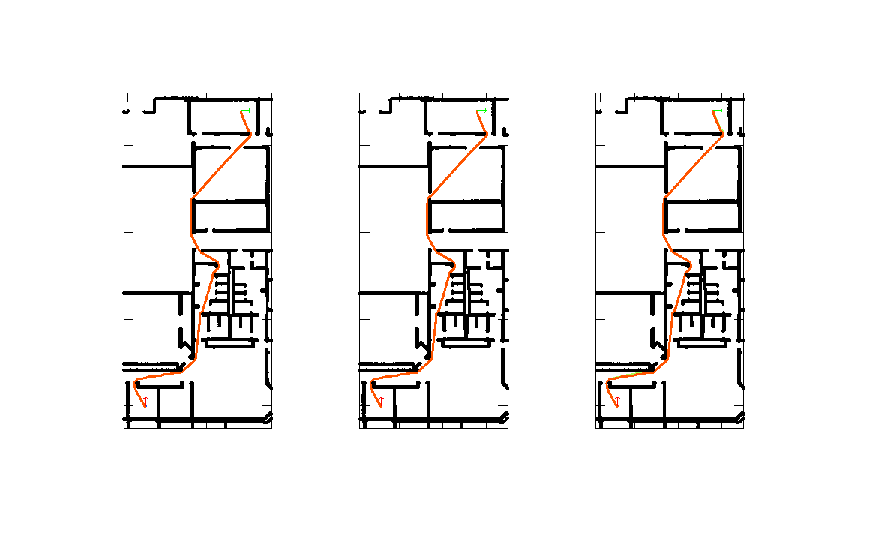
\includegraphics{./figures/parts/02/chapters/01/sections/04/global_plan_navfn_willowgarage}}%
    \gplfronttext
  \end{picture}%
\endgroup

  \end{subfigure}%
  \vspace{-1.5cm}
  \begin{subfigure}[t]{\linewidth}
    \centering
    % GNUPLOT: LaTeX picture with Postscript
\begingroup
  \makeatletter
  \providecommand\color[2][]{%
    \GenericError{(gnuplot) \space\space\space\@spaces}{%
      Package color not loaded in conjunction with
      terminal option `colourtext'%
    }{See the gnuplot documentation for explanation.%
    }{Either use 'blacktext' in gnuplot or load the package
      color.sty in LaTeX.}%
    \renewcommand\color[2][]{}%
  }%
  \providecommand\includegraphics[2][]{%
    \GenericError{(gnuplot) \space\space\space\@spaces}{%
      Package graphicx or graphics not loaded%
    }{See the gnuplot documentation for explanation.%
    }{The gnuplot epslatex terminal needs graphicx.sty or graphics.sty.}%
    \renewcommand\includegraphics[2][]{}%
  }%
  \providecommand\rotatebox[2]{#2}%
  \@ifundefined{ifGPcolor}{%
    \newif\ifGPcolor
    \GPcolorfalse
  }{}%
  \@ifundefined{ifGPblacktext}{%
    \newif\ifGPblacktext
    \GPblacktexttrue
  }{}%
  % define a \g@addto@macro without @ in the name:
  \let\gplgaddtomacro\g@addto@macro
  % define empty templates for all commands taking text:
  \gdef\gplfronttext{}%
  \gdef\gplfronttext{}%
  \makeatother
  \ifGPblacktext
    % no textcolor at all
    \def\colorrgb#1{}%
    \def\colorgray#1{}%
  \else
    % gray or color?
    \ifGPcolor
      \def\colorrgb#1{\color[rgb]{#1}}%
      \def\colorgray#1{\color[gray]{#1}}%
      \expandafter\def\csname LTw\endcsname{\color{white}}%
      \expandafter\def\csname LTb\endcsname{\color{black}}%
      \expandafter\def\csname LTa\endcsname{\color{black}}%
      \expandafter\def\csname LT0\endcsname{\color[rgb]{1,0,0}}%
      \expandafter\def\csname LT1\endcsname{\color[rgb]{0,1,0}}%
      \expandafter\def\csname LT2\endcsname{\color[rgb]{0,0,1}}%
      \expandafter\def\csname LT3\endcsname{\color[rgb]{1,0,1}}%
      \expandafter\def\csname LT4\endcsname{\color[rgb]{0,1,1}}%
      \expandafter\def\csname LT5\endcsname{\color[rgb]{1,1,0}}%
      \expandafter\def\csname LT6\endcsname{\color[rgb]{0,0,0}}%
      \expandafter\def\csname LT7\endcsname{\color[rgb]{1,0.3,0}}%
      \expandafter\def\csname LT8\endcsname{\color[rgb]{0.5,0.5,0.5}}%
    \else
      % gray
      \def\colorrgb#1{\color{black}}%
      \def\colorgray#1{\color[gray]{#1}}%
      \expandafter\def\csname LTw\endcsname{\color{white}}%
      \expandafter\def\csname LTb\endcsname{\color{black}}%
      \expandafter\def\csname LTa\endcsname{\color{black}}%
      \expandafter\def\csname LT0\endcsname{\color{black}}%
      \expandafter\def\csname LT1\endcsname{\color{black}}%
      \expandafter\def\csname LT2\endcsname{\color{black}}%
      \expandafter\def\csname LT3\endcsname{\color{black}}%
      \expandafter\def\csname LT4\endcsname{\color{black}}%
      \expandafter\def\csname LT5\endcsname{\color{black}}%
      \expandafter\def\csname LT6\endcsname{\color{black}}%
      \expandafter\def\csname LT7\endcsname{\color{black}}%
      \expandafter\def\csname LT8\endcsname{\color{black}}%
    \fi
  \fi
  \setlength{\unitlength}{0.0500bp}%
  \begin{picture}(8000.00,4800.00)%
    \gplgaddtomacro\gplfronttext{%
      \colorrgb{0.00,0.00,0.00}%
      \put(891,1073){\makebox(0,0)[r]{\strut{}$45$}}%
      \colorrgb{0.00,0.00,0.00}%
      \put(891,1490){\makebox(0,0)[r]{\strut{}$50$}}%
      \colorrgb{0.00,0.00,0.00}%
      \put(891,1908){\makebox(0,0)[r]{\strut{}$55$}}%
      \colorrgb{0.00,0.00,0.00}%
      \put(891,2325){\makebox(0,0)[r]{\strut{}$60$}}%
      \colorrgb{0.00,0.00,0.00}%
      \put(891,2743){\makebox(0,0)[r]{\strut{}$65$}}%
      \colorrgb{0.00,0.00,0.00}%
      \put(891,3160){\makebox(0,0)[r]{\strut{}$70$}}%
      \colorrgb{0.00,0.00,0.00}%
      \put(891,3578){\makebox(0,0)[r]{\strut{}$75$}}%
      \colorrgb{0.00,0.00,0.00}%
      \put(891,3995){\makebox(0,0)[r]{\strut{}$80$}}%
      \colorrgb{0.00,0.00,0.00}%
      \put(1065,644){\makebox(0,0){\strut{}$56$}}%
      \colorrgb{0.00,0.00,0.00}%
      \put(1399,644){\makebox(0,0){\strut{}$60$}}%
      \colorrgb{0.00,0.00,0.00}%
      \put(1817,644){\makebox(0,0){\strut{}$65$}}%
      \colorrgb{0.00,0.00,0.00}%
      \put(2234,644){\makebox(0,0){\strut{}$70$}}%
      \colorrgb{0.00,0.00,0.00}%
      \put(385,2471){\rotatebox{90}{\makebox(0,0){\strut{}$y$ [m]}}}%
      \colorrgb{0.00,0.00,0.00}%
      \put(1733,314){\makebox(0,0){\strut{}$x$ [m]}}%
      \colorrgb{0.00,0.00,0.00}%
      \put(1433,4409){\makebox(0,0){\strut{}\texttt{global\_planner} / \texttt{dwa}}}%
    }%
    \gplgaddtomacro\gplfronttext{%
    }%
    \gplgaddtomacro\gplfronttext{%
      \put(3331,644){\makebox(0,0){\strut{}$56$}}%
      \colorrgb{0.00,0.00,0.00}%
      \put(3665,644){\makebox(0,0){\strut{}$60$}}%
      \colorrgb{0.00,0.00,0.00}%
      \put(4083,644){\makebox(0,0){\strut{}$65$}}%
      \colorrgb{0.00,0.00,0.00}%
      \put(4500,644){\makebox(0,0){\strut{}$70$}}%
      \colorrgb{0.00,0.00,0.00}%
      \put(3999,314){\makebox(0,0){\strut{}$x$ [m]}}%
      \colorrgb{0.00,0.00,0.00}%
      \put(3999,4409){\makebox(0,0){\strut{}\texttt{global\_planner} / \texttt{eband}}}%
    }%
    \gplgaddtomacro\gplfronttext{%
    }%
    \gplgaddtomacro\gplfronttext{%
      \put(5598,644){\makebox(0,0){\strut{}$56$}}%
      \colorrgb{0.00,0.00,0.00}%
      \put(5932,644){\makebox(0,0){\strut{}$60$}}%
      \colorrgb{0.00,0.00,0.00}%
      \put(6349,644){\makebox(0,0){\strut{}$65$}}%
      \colorrgb{0.00,0.00,0.00}%
      \put(6766,644){\makebox(0,0){\strut{}$70$}}%
      \colorrgb{0.00,0.00,0.00}%
      \put(6265,314){\makebox(0,0){\strut{}$x$ [m]}}%
      \colorrgb{0.00,0.00,0.00}%
      \put(6565,4409){\makebox(0,0){\strut{}\texttt{global\_planner} / \texttt{teb}}}%
    }%
    \gplgaddtomacro\gplfronttext{%
    }%
    \put(0,0){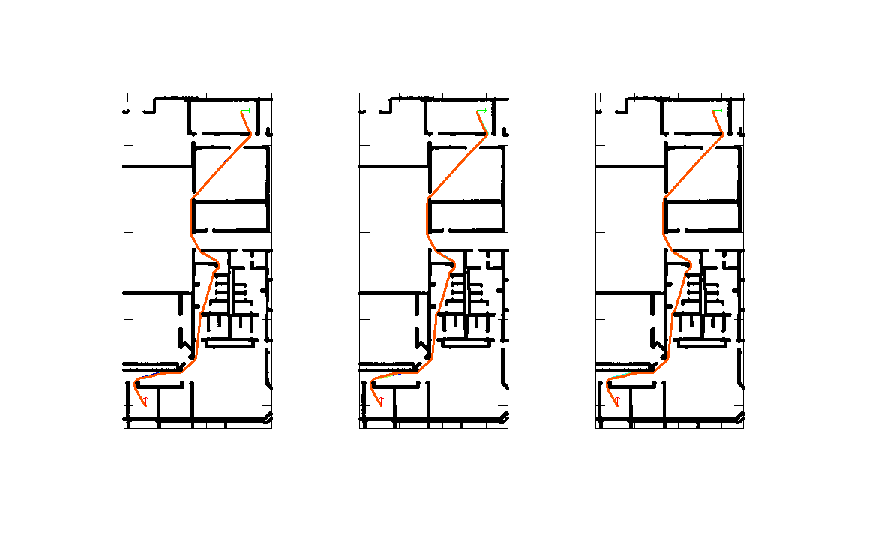
\includegraphics{./figures/parts/02/chapters/01/sections/04/global_plan_globalplanner_willowgarage}}%
    \gplfronttext
  \end{picture}%
\endgroup

  \end{subfigure}%
  \vspace{-1.5cm}
  \begin{subfigure}[t]{\linewidth}
    \centering
    % GNUPLOT: LaTeX picture with Postscript
\begingroup
  \makeatletter
  \providecommand\color[2][]{%
    \GenericError{(gnuplot) \space\space\space\@spaces}{%
      Package color not loaded in conjunction with
      terminal option `colourtext'%
    }{See the gnuplot documentation for explanation.%
    }{Either use 'blacktext' in gnuplot or load the package
      color.sty in LaTeX.}%
    \renewcommand\color[2][]{}%
  }%
  \providecommand\includegraphics[2][]{%
    \GenericError{(gnuplot) \space\space\space\@spaces}{%
      Package graphicx or graphics not loaded%
    }{See the gnuplot documentation for explanation.%
    }{The gnuplot epslatex terminal needs graphicx.sty or graphics.sty.}%
    \renewcommand\includegraphics[2][]{}%
  }%
  \providecommand\rotatebox[2]{#2}%
  \@ifundefined{ifGPcolor}{%
    \newif\ifGPcolor
    \GPcolorfalse
  }{}%
  \@ifundefined{ifGPblacktext}{%
    \newif\ifGPblacktext
    \GPblacktexttrue
  }{}%
  % define a \g@addto@macro without @ in the name:
  \let\gplgaddtomacro\g@addto@macro
  % define empty templates for all commands taking text:
  \gdef\gplfronttext{}%
  \gdef\gplfronttext{}%
  \makeatother
  \ifGPblacktext
    % no textcolor at all
    \def\colorrgb#1{}%
    \def\colorgray#1{}%
  \else
    % gray or color?
    \ifGPcolor
      \def\colorrgb#1{\color[rgb]{#1}}%
      \def\colorgray#1{\color[gray]{#1}}%
      \expandafter\def\csname LTw\endcsname{\color{white}}%
      \expandafter\def\csname LTb\endcsname{\color{black}}%
      \expandafter\def\csname LTa\endcsname{\color{black}}%
      \expandafter\def\csname LT0\endcsname{\color[rgb]{1,0,0}}%
      \expandafter\def\csname LT1\endcsname{\color[rgb]{0,1,0}}%
      \expandafter\def\csname LT2\endcsname{\color[rgb]{0,0,1}}%
      \expandafter\def\csname LT3\endcsname{\color[rgb]{1,0,1}}%
      \expandafter\def\csname LT4\endcsname{\color[rgb]{0,1,1}}%
      \expandafter\def\csname LT5\endcsname{\color[rgb]{1,1,0}}%
      \expandafter\def\csname LT6\endcsname{\color[rgb]{0,0,0}}%
      \expandafter\def\csname LT7\endcsname{\color[rgb]{1,0.3,0}}%
      \expandafter\def\csname LT8\endcsname{\color[rgb]{0.5,0.5,0.5}}%
    \else
      % gray
      \def\colorrgb#1{\color{black}}%
      \def\colorgray#1{\color[gray]{#1}}%
      \expandafter\def\csname LTw\endcsname{\color{white}}%
      \expandafter\def\csname LTb\endcsname{\color{black}}%
      \expandafter\def\csname LTa\endcsname{\color{black}}%
      \expandafter\def\csname LT0\endcsname{\color{black}}%
      \expandafter\def\csname LT1\endcsname{\color{black}}%
      \expandafter\def\csname LT2\endcsname{\color{black}}%
      \expandafter\def\csname LT3\endcsname{\color{black}}%
      \expandafter\def\csname LT4\endcsname{\color{black}}%
      \expandafter\def\csname LT5\endcsname{\color{black}}%
      \expandafter\def\csname LT6\endcsname{\color{black}}%
      \expandafter\def\csname LT7\endcsname{\color{black}}%
      \expandafter\def\csname LT8\endcsname{\color{black}}%
    \fi
  \fi
  \setlength{\unitlength}{0.0500bp}%
  \begin{picture}(8000.00,4800.00)%
    \gplgaddtomacro\gplfronttext{%
      \colorrgb{0.00,0.00,0.00}%
      \put(891,1073){\makebox(0,0)[r]{\strut{}$45$}}%
      \colorrgb{0.00,0.00,0.00}%
      \put(891,1490){\makebox(0,0)[r]{\strut{}$50$}}%
      \colorrgb{0.00,0.00,0.00}%
      \put(891,1908){\makebox(0,0)[r]{\strut{}$55$}}%
      \colorrgb{0.00,0.00,0.00}%
      \put(891,2325){\makebox(0,0)[r]{\strut{}$60$}}%
      \colorrgb{0.00,0.00,0.00}%
      \put(891,2743){\makebox(0,0)[r]{\strut{}$65$}}%
      \colorrgb{0.00,0.00,0.00}%
      \put(891,3160){\makebox(0,0)[r]{\strut{}$70$}}%
      \colorrgb{0.00,0.00,0.00}%
      \put(891,3578){\makebox(0,0)[r]{\strut{}$75$}}%
      \colorrgb{0.00,0.00,0.00}%
      \put(891,3995){\makebox(0,0)[r]{\strut{}$80$}}%
      \colorrgb{0.00,0.00,0.00}%
      \put(1065,644){\makebox(0,0){\strut{}$56$}}%
      \colorrgb{0.00,0.00,0.00}%
      \put(1399,644){\makebox(0,0){\strut{}$60$}}%
      \colorrgb{0.00,0.00,0.00}%
      \put(1817,644){\makebox(0,0){\strut{}$65$}}%
      \colorrgb{0.00,0.00,0.00}%
      \put(2234,644){\makebox(0,0){\strut{}$70$}}%
      \colorrgb{0.00,0.00,0.00}%
      \put(385,2471){\rotatebox{90}{\makebox(0,0){\strut{}$y$ [m]}}}%
      \colorrgb{0.00,0.00,0.00}%
      \put(1733,314){\makebox(0,0){\strut{}$x$ [m]}}%
      \colorrgb{0.00,0.00,0.00}%
      \put(1733,4409){\makebox(0,0){\strut{}\texttt{sbpl} / \texttt{dwa}}}%
    }%
    \gplgaddtomacro\gplfronttext{%
    }%
    \gplgaddtomacro\gplfronttext{%
      \colorrgb{0.00,0.00,0.00}%
      \put(3157,1073){\makebox(0,0)[r]{\strut{}$45$}}%
      \colorrgb{0.00,0.00,0.00}%
      \put(3157,1490){\makebox(0,0)[r]{\strut{}$50$}}%
      \colorrgb{0.00,0.00,0.00}%
      \put(3157,1908){\makebox(0,0)[r]{\strut{}$55$}}%
      \colorrgb{0.00,0.00,0.00}%
      \put(3157,2325){\makebox(0,0)[r]{\strut{}$60$}}%
      \colorrgb{0.00,0.00,0.00}%
      \put(3157,2743){\makebox(0,0)[r]{\strut{}$65$}}%
      \colorrgb{0.00,0.00,0.00}%
      \put(3157,3160){\makebox(0,0)[r]{\strut{}$70$}}%
      \colorrgb{0.00,0.00,0.00}%
      \put(3157,3578){\makebox(0,0)[r]{\strut{}$75$}}%
      \colorrgb{0.00,0.00,0.00}%
      \put(3157,3995){\makebox(0,0)[r]{\strut{}$80$}}%
      \colorrgb{0.00,0.00,0.00}%
      \put(3331,644){\makebox(0,0){\strut{}$56$}}%
      \colorrgb{0.00,0.00,0.00}%
      \put(3665,644){\makebox(0,0){\strut{}$60$}}%
      \colorrgb{0.00,0.00,0.00}%
      \put(4083,644){\makebox(0,0){\strut{}$65$}}%
      \colorrgb{0.00,0.00,0.00}%
      \put(4500,644){\makebox(0,0){\strut{}$70$}}%
      \colorrgb{0.00,0.00,0.00}%
      \put(3999,314){\makebox(0,0){\strut{}$x$ [m]}}%
      \colorrgb{0.00,0.00,0.00}%
      \put(3999,4409){\makebox(0,0){\strut{}\texttt{sbpl} / \texttt{eband}}}%
    }%
    \gplgaddtomacro\gplfronttext{%
    }%
    \gplgaddtomacro\gplfronttext{%
      \colorrgb{0.00,0.00,0.00}%
      \put(5424,1073){\makebox(0,0)[r]{\strut{}$45$}}%
      \colorrgb{0.00,0.00,0.00}%
      \put(5424,1490){\makebox(0,0)[r]{\strut{}$50$}}%
      \colorrgb{0.00,0.00,0.00}%
      \put(5424,1908){\makebox(0,0)[r]{\strut{}$55$}}%
      \colorrgb{0.00,0.00,0.00}%
      \put(5424,2325){\makebox(0,0)[r]{\strut{}$60$}}%
      \colorrgb{0.00,0.00,0.00}%
      \put(5424,2743){\makebox(0,0)[r]{\strut{}$65$}}%
      \colorrgb{0.00,0.00,0.00}%
      \put(5424,3160){\makebox(0,0)[r]{\strut{}$70$}}%
      \colorrgb{0.00,0.00,0.00}%
      \put(5424,3578){\makebox(0,0)[r]{\strut{}$75$}}%
      \colorrgb{0.00,0.00,0.00}%
      \put(5424,3995){\makebox(0,0)[r]{\strut{}$80$}}%
      \colorrgb{0.00,0.00,0.00}%
      \put(5598,644){\makebox(0,0){\strut{}$56$}}%
      \colorrgb{0.00,0.00,0.00}%
      \put(5932,644){\makebox(0,0){\strut{}$60$}}%
      \colorrgb{0.00,0.00,0.00}%
      \put(6349,644){\makebox(0,0){\strut{}$65$}}%
      \colorrgb{0.00,0.00,0.00}%
      \put(6766,644){\makebox(0,0){\strut{}$70$}}%
      \colorrgb{0.00,0.00,0.00}%
      \put(6265,314){\makebox(0,0){\strut{}$x$ [m]}}%
      \colorrgb{0.00,0.00,0.00}%
      \put(6265,4409){\makebox(0,0){\strut{}\texttt{sbpl} / \texttt{teb}}}%
    }%
    \gplgaddtomacro\gplfronttext{%
    }%
    \gplfronttext
    \put(0,0){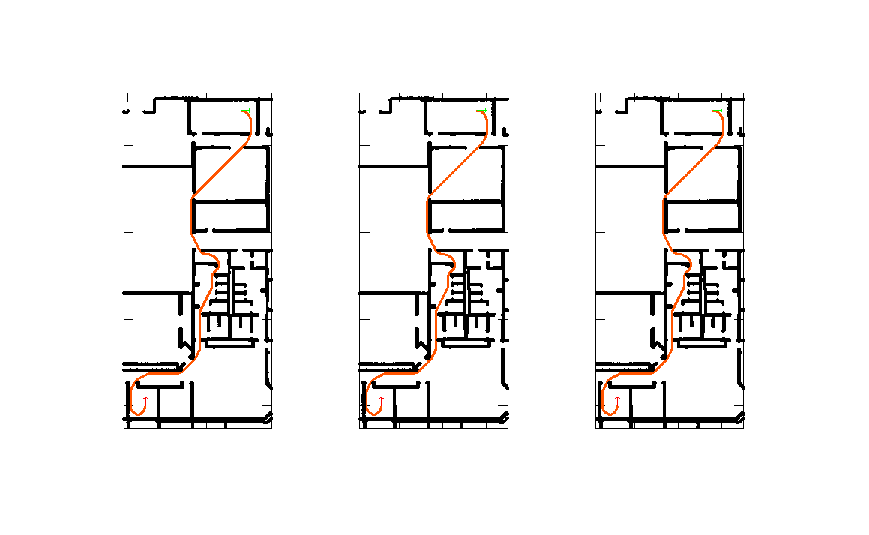
\includegraphics{./figures/parts/02/chapters/01/sections/04/global_plan_sbpl_willowgarage}}%
    \gplfronttext
  \end{picture}%
\endgroup

  \end{subfigure}%
  \caption{\small Τα σχεδιασθέντα μονοπάτια προς ακολούθηση $\bm{\mathcal{G}}$
           που παρήχθησαν από τους τρεις αλγορίθμους χάραξης μονοπατιών για
           κάθε συνδυασμό τους με ελεγκτή κίνησης του πίνακα
           \ref{tbl:planners_sifted_list}, σε σχέση με τις ορισμένες αρχικές και
           τελικές στάσεις του περιβάλλοντος WILLOWGARAGE}
  \label{fig:global_plans:willowgarage}
\end{figure}

Το σχήμα \ref{fig:ground_truths:willowgarage} απεικονίζει τις πραγματικές
διαδρομές που διένυσε το ρομπότ για όλους τους συνδυασμούς αλγορίθμων σχεδίασης
μονοπατιών και ελεγκτών κίνησης του ίδιου πίνακα, για $N=10$ προσομοιώσεις για
κάθε συνδυασμό.

\begin{figure}
\raggedright
  \begin{subfigure}[t]{\linewidth}
    \centering
    % GNUPLOT: LaTeX picture with Postscript
\begingroup
  \makeatletter
  \providecommand\color[2][]{%
    \GenericError{(gnuplot) \space\space\space\@spaces}{%
      Package color not loaded in conjunction with
      terminal option `colourtext'%
    }{See the gnuplot documentation for explanation.%
    }{Either use 'blacktext' in gnuplot or load the package
      color.sty in LaTeX.}%
    \renewcommand\color[2][]{}%
  }%
  \providecommand\includegraphics[2][]{%
    \GenericError{(gnuplot) \space\space\space\@spaces}{%
      Package graphicx or graphics not loaded%
    }{See the gnuplot documentation for explanation.%
    }{The gnuplot epslatex terminal needs graphicx.sty or graphics.sty.}%
    \renewcommand\includegraphics[2][]{}%
  }%
  \providecommand\rotatebox[2]{#2}%
  \@ifundefined{ifGPcolor}{%
    \newif\ifGPcolor
    \GPcolorfalse
  }{}%
  \@ifundefined{ifGPblacktext}{%
    \newif\ifGPblacktext
    \GPblacktexttrue
  }{}%
  % define a \g@addto@macro without @ in the name:
  \let\gplgaddtomacro\g@addto@macro
  % define empty templates for all commands taking text:
  \gdef\gplfronttext{}%
  \gdef\gplfronttext{}%
  \makeatother
  \ifGPblacktext
    % no textcolor at all
    \def\colorrgb#1{}%
    \def\colorgray#1{}%
  \else
    % gray or color?
    \ifGPcolor
      \def\colorrgb#1{\color[rgb]{#1}}%
      \def\colorgray#1{\color[gray]{#1}}%
      \expandafter\def\csname LTw\endcsname{\color{white}}%
      \expandafter\def\csname LTb\endcsname{\color{black}}%
      \expandafter\def\csname LTa\endcsname{\color{black}}%
      \expandafter\def\csname LT0\endcsname{\color[rgb]{1,0,0}}%
      \expandafter\def\csname LT1\endcsname{\color[rgb]{0,1,0}}%
      \expandafter\def\csname LT2\endcsname{\color[rgb]{0,0,1}}%
      \expandafter\def\csname LT3\endcsname{\color[rgb]{1,0,1}}%
      \expandafter\def\csname LT4\endcsname{\color[rgb]{0,1,1}}%
      \expandafter\def\csname LT5\endcsname{\color[rgb]{1,1,0}}%
      \expandafter\def\csname LT6\endcsname{\color[rgb]{0,0,0}}%
      \expandafter\def\csname LT7\endcsname{\color[rgb]{1,0.3,0}}%
      \expandafter\def\csname LT8\endcsname{\color[rgb]{0.5,0.5,0.5}}%
    \else
      % gray
      \def\colorrgb#1{\color{black}}%
      \def\colorgray#1{\color[gray]{#1}}%
      \expandafter\def\csname LTw\endcsname{\color{white}}%
      \expandafter\def\csname LTb\endcsname{\color{black}}%
      \expandafter\def\csname LTa\endcsname{\color{black}}%
      \expandafter\def\csname LT0\endcsname{\color{black}}%
      \expandafter\def\csname LT1\endcsname{\color{black}}%
      \expandafter\def\csname LT2\endcsname{\color{black}}%
      \expandafter\def\csname LT3\endcsname{\color{black}}%
      \expandafter\def\csname LT4\endcsname{\color{black}}%
      \expandafter\def\csname LT5\endcsname{\color{black}}%
      \expandafter\def\csname LT6\endcsname{\color{black}}%
      \expandafter\def\csname LT7\endcsname{\color{black}}%
      \expandafter\def\csname LT8\endcsname{\color{black}}%
    \fi
  \fi
  \setlength{\unitlength}{0.0500bp}%
  \begin{picture}(8000.00,4800.00)%
    \gplgaddtomacro\gplfronttext{%
      \colorrgb{0.00,0.00,0.00}%
      \put(891,1073){\makebox(0,0)[r]{\strut{}$45$}}%
      \colorrgb{0.00,0.00,0.00}%
      \put(891,1490){\makebox(0,0)[r]{\strut{}$50$}}%
      \colorrgb{0.00,0.00,0.00}%
      \put(891,1908){\makebox(0,0)[r]{\strut{}$55$}}%
      \colorrgb{0.00,0.00,0.00}%
      \put(891,2325){\makebox(0,0)[r]{\strut{}$60$}}%
      \colorrgb{0.00,0.00,0.00}%
      \put(891,2743){\makebox(0,0)[r]{\strut{}$65$}}%
      \colorrgb{0.00,0.00,0.00}%
      \put(891,3160){\makebox(0,0)[r]{\strut{}$70$}}%
      \colorrgb{0.00,0.00,0.00}%
      \put(891,3578){\makebox(0,0)[r]{\strut{}$75$}}%
      \colorrgb{0.00,0.00,0.00}%
      \put(891,3995){\makebox(0,0)[r]{\strut{}$80$}}%
      \colorrgb{0.00,0.00,0.00}%
      \put(1065,644){\makebox(0,0){\strut{}$56$}}%
      \colorrgb{0.00,0.00,0.00}%
      \put(1399,644){\makebox(0,0){\strut{}$60$}}%
      \colorrgb{0.00,0.00,0.00}%
      \put(1817,644){\makebox(0,0){\strut{}$65$}}%
      \colorrgb{0.00,0.00,0.00}%
      \put(2234,644){\makebox(0,0){\strut{}$70$}}%
      \colorrgb{0.00,0.00,0.00}%
      \put(385,2471){\rotatebox{90}{\makebox(0,0){\strut{}y [m]}}}%
      \colorrgb{0.00,0.00,0.00}%
      \put(1733,314){\makebox(0,0){\strut{}x [m]}}%
      \colorrgb{0.00,0.00,0.00}%
      \put(1733,4409){\makebox(0,0){\strut{}\texttt{navfn} / \texttt{dwa}}}%
    }%
    \gplgaddtomacro\gplfronttext{%
    }%
    \gplgaddtomacro\gplfronttext{%
      \put(3331,644){\makebox(0,0){\strut{}$56$}}%
      \colorrgb{0.00,0.00,0.00}%
      \put(3665,644){\makebox(0,0){\strut{}$60$}}%
      \colorrgb{0.00,0.00,0.00}%
      \put(4083,644){\makebox(0,0){\strut{}$65$}}%
      \colorrgb{0.00,0.00,0.00}%
      \put(4500,644){\makebox(0,0){\strut{}$70$}}%
      \colorrgb{0.00,0.00,0.00}%
      \put(3999,314){\makebox(0,0){\strut{}x [m]}}%
      \colorrgb{0.00,0.00,0.00}%
      \put(3999,4409){\makebox(0,0){\strut{}\texttt{navfn} / \texttt{eband}}}%
    }%
    \gplgaddtomacro\gplfronttext{%
    }%
    \gplgaddtomacro\gplfronttext{%
      \put(5598,644){\makebox(0,0){\strut{}$56$}}%
      \colorrgb{0.00,0.00,0.00}%
      \put(5932,644){\makebox(0,0){\strut{}$60$}}%
      \colorrgb{0.00,0.00,0.00}%
      \put(6349,644){\makebox(0,0){\strut{}$65$}}%
      \colorrgb{0.00,0.00,0.00}%
      \put(6766,644){\makebox(0,0){\strut{}$70$}}%
      \colorrgb{0.00,0.00,0.00}%
      \put(6265,314){\makebox(0,0){\strut{}x [m]}}%
      \colorrgb{0.00,0.00,0.00}%
      \put(6265,4409){\makebox(0,0){\strut{}\texttt{navfn} / \texttt{teb}}}%
    }%
    \gplgaddtomacro\gplfronttext{%
    }%
    \put(0,0){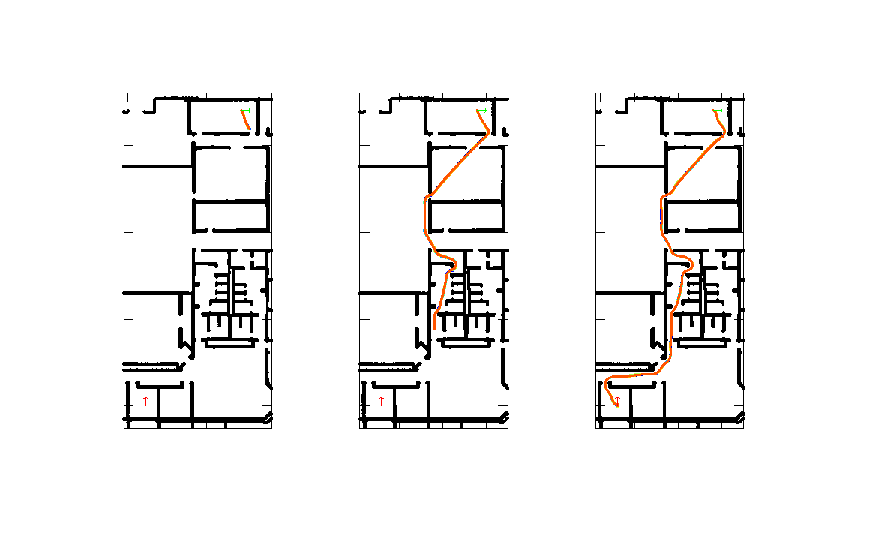
\includegraphics{./figures/parts/02/chapters/01/sections/04/ground_truth_navfn_willowgarage}}%
    \gplfronttext
  \end{picture}%
\endgroup

  \end{subfigure}%
  \vspace{-1.5cm}
  \begin{subfigure}[t]{\linewidth}
    \centering
    % GNUPLOT: LaTeX picture with Postscript
\begingroup
  \makeatletter
  \providecommand\color[2][]{%
    \GenericError{(gnuplot) \space\space\space\@spaces}{%
      Package color not loaded in conjunction with
      terminal option `colourtext'%
    }{See the gnuplot documentation for explanation.%
    }{Either use 'blacktext' in gnuplot or load the package
      color.sty in LaTeX.}%
    \renewcommand\color[2][]{}%
  }%
  \providecommand\includegraphics[2][]{%
    \GenericError{(gnuplot) \space\space\space\@spaces}{%
      Package graphicx or graphics not loaded%
    }{See the gnuplot documentation for explanation.%
    }{The gnuplot epslatex terminal needs graphicx.sty or graphics.sty.}%
    \renewcommand\includegraphics[2][]{}%
  }%
  \providecommand\rotatebox[2]{#2}%
  \@ifundefined{ifGPcolor}{%
    \newif\ifGPcolor
    \GPcolorfalse
  }{}%
  \@ifundefined{ifGPblacktext}{%
    \newif\ifGPblacktext
    \GPblacktexttrue
  }{}%
  % define a \g@addto@macro without @ in the name:
  \let\gplgaddtomacro\g@addto@macro
  % define empty templates for all commands taking text:
  \gdef\gplfronttext{}%
  \gdef\gplfronttext{}%
  \makeatother
  \ifGPblacktext
    % no textcolor at all
    \def\colorrgb#1{}%
    \def\colorgray#1{}%
  \else
    % gray or color?
    \ifGPcolor
      \def\colorrgb#1{\color[rgb]{#1}}%
      \def\colorgray#1{\color[gray]{#1}}%
      \expandafter\def\csname LTw\endcsname{\color{white}}%
      \expandafter\def\csname LTb\endcsname{\color{black}}%
      \expandafter\def\csname LTa\endcsname{\color{black}}%
      \expandafter\def\csname LT0\endcsname{\color[rgb]{1,0,0}}%
      \expandafter\def\csname LT1\endcsname{\color[rgb]{0,1,0}}%
      \expandafter\def\csname LT2\endcsname{\color[rgb]{0,0,1}}%
      \expandafter\def\csname LT3\endcsname{\color[rgb]{1,0,1}}%
      \expandafter\def\csname LT4\endcsname{\color[rgb]{0,1,1}}%
      \expandafter\def\csname LT5\endcsname{\color[rgb]{1,1,0}}%
      \expandafter\def\csname LT6\endcsname{\color[rgb]{0,0,0}}%
      \expandafter\def\csname LT7\endcsname{\color[rgb]{1,0.3,0}}%
      \expandafter\def\csname LT8\endcsname{\color[rgb]{0.5,0.5,0.5}}%
    \else
      % gray
      \def\colorrgb#1{\color{black}}%
      \def\colorgray#1{\color[gray]{#1}}%
      \expandafter\def\csname LTw\endcsname{\color{white}}%
      \expandafter\def\csname LTb\endcsname{\color{black}}%
      \expandafter\def\csname LTa\endcsname{\color{black}}%
      \expandafter\def\csname LT0\endcsname{\color{black}}%
      \expandafter\def\csname LT1\endcsname{\color{black}}%
      \expandafter\def\csname LT2\endcsname{\color{black}}%
      \expandafter\def\csname LT3\endcsname{\color{black}}%
      \expandafter\def\csname LT4\endcsname{\color{black}}%
      \expandafter\def\csname LT5\endcsname{\color{black}}%
      \expandafter\def\csname LT6\endcsname{\color{black}}%
      \expandafter\def\csname LT7\endcsname{\color{black}}%
      \expandafter\def\csname LT8\endcsname{\color{black}}%
    \fi
  \fi
  \setlength{\unitlength}{0.0500bp}%
  \begin{picture}(8000.00,4800.00)%
    \gplgaddtomacro\gplfronttext{%
      \colorrgb{0.00,0.00,0.00}%
      \put(891,1073){\makebox(0,0)[r]{\strut{}$45$}}%
      \colorrgb{0.00,0.00,0.00}%
      \put(891,1490){\makebox(0,0)[r]{\strut{}$50$}}%
      \colorrgb{0.00,0.00,0.00}%
      \put(891,1908){\makebox(0,0)[r]{\strut{}$55$}}%
      \colorrgb{0.00,0.00,0.00}%
      \put(891,2325){\makebox(0,0)[r]{\strut{}$60$}}%
      \colorrgb{0.00,0.00,0.00}%
      \put(891,2743){\makebox(0,0)[r]{\strut{}$65$}}%
      \colorrgb{0.00,0.00,0.00}%
      \put(891,3160){\makebox(0,0)[r]{\strut{}$70$}}%
      \colorrgb{0.00,0.00,0.00}%
      \put(891,3578){\makebox(0,0)[r]{\strut{}$75$}}%
      \colorrgb{0.00,0.00,0.00}%
      \put(891,3995){\makebox(0,0)[r]{\strut{}$80$}}%
      \colorrgb{0.00,0.00,0.00}%
      \put(1065,644){\makebox(0,0){\strut{}$56$}}%
      \colorrgb{0.00,0.00,0.00}%
      \put(1399,644){\makebox(0,0){\strut{}$60$}}%
      \colorrgb{0.00,0.00,0.00}%
      \put(1817,644){\makebox(0,0){\strut{}$65$}}%
      \colorrgb{0.00,0.00,0.00}%
      \put(2234,644){\makebox(0,0){\strut{}$70$}}%
      \colorrgb{0.00,0.00,0.00}%
      \put(385,2471){\rotatebox{90}{\makebox(0,0){\strut{}y [m]}}}%
      \colorrgb{0.00,0.00,0.00}%
      \put(1733,314){\makebox(0,0){\strut{}$x$ [m]}}%
      \colorrgb{0.00,0.00,0.00}%
      \put(1433,4409){\makebox(0,0){\strut{}\texttt{global\_planner} / \texttt{dwa}}}%
    }%
    \gplgaddtomacro\gplfronttext{%
    }%
    \gplgaddtomacro\gplfronttext{%
      \colorrgb{0.00,0.00,0.00}%
      \put(3331,644){\makebox(0,0){\strut{}$56$}}%
      \colorrgb{0.00,0.00,0.00}%
      \put(3665,644){\makebox(0,0){\strut{}$60$}}%
      \colorrgb{0.00,0.00,0.00}%
      \put(4083,644){\makebox(0,0){\strut{}$65$}}%
      \colorrgb{0.00,0.00,0.00}%
      \put(4500,644){\makebox(0,0){\strut{}$70$}}%
      \colorrgb{0.00,0.00,0.00}%
      \put(3999,314){\makebox(0,0){\strut{}$x$ [m]}}%
      \colorrgb{0.00,0.00,0.00}%
      \put(3999,4409){\makebox(0,0){\strut{}\texttt{global\_planner} / \texttt{eband}}}%
    }%
    \gplgaddtomacro\gplfronttext{%
    }%
    \gplgaddtomacro\gplfronttext{%
      \colorrgb{0.00,0.00,0.00}%
      \put(5598,644){\makebox(0,0){\strut{}$56$}}%
      \colorrgb{0.00,0.00,0.00}%
      \put(5932,644){\makebox(0,0){\strut{}$60$}}%
      \colorrgb{0.00,0.00,0.00}%
      \put(6349,644){\makebox(0,0){\strut{}$65$}}%
      \colorrgb{0.00,0.00,0.00}%
      \put(6766,644){\makebox(0,0){\strut{}$70$}}%
      \colorrgb{0.00,0.00,0.00}%
      \put(6265,314){\makebox(0,0){\strut{}$x$ [m]}}%
      \colorrgb{0.00,0.00,0.00}%
      \put(6565,4409){\makebox(0,0){\strut{}\texttt{global\_planner} / \texttt{teb}}}%
    }%
    \gplgaddtomacro\gplfronttext{%
    }%
    \gplfronttext
    \put(0,0){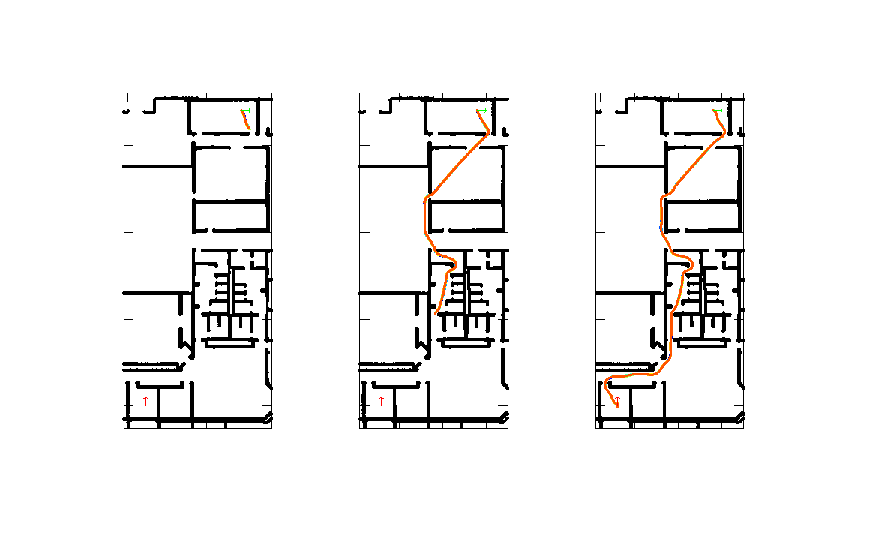
\includegraphics{./figures/parts/02/chapters/01/sections/04/ground_truth_globalplanner_willowgarage}}%
    \gplfronttext
  \end{picture}%
\endgroup

  \end{subfigure}%
  \vspace{-1.5cm}
  \begin{subfigure}[t]{\linewidth}
    \centering
    % GNUPLOT: LaTeX picture with Postscript
\begingroup
  \makeatletter
  \providecommand\color[2][]{%
    \GenericError{(gnuplot) \space\space\space\@spaces}{%
      Package color not loaded in conjunction with
      terminal option `colourtext'%
    }{See the gnuplot documentation for explanation.%
    }{Either use 'blacktext' in gnuplot or load the package
      color.sty in LaTeX.}%
    \renewcommand\color[2][]{}%
  }%
  \providecommand\includegraphics[2][]{%
    \GenericError{(gnuplot) \space\space\space\@spaces}{%
      Package graphicx or graphics not loaded%
    }{See the gnuplot documentation for explanation.%
    }{The gnuplot epslatex terminal needs graphicx.sty or graphics.sty.}%
    \renewcommand\includegraphics[2][]{}%
  }%
  \providecommand\rotatebox[2]{#2}%
  \@ifundefined{ifGPcolor}{%
    \newif\ifGPcolor
    \GPcolorfalse
  }{}%
  \@ifundefined{ifGPblacktext}{%
    \newif\ifGPblacktext
    \GPblacktexttrue
  }{}%
  % define a \g@addto@macro without @ in the name:
  \let\gplgaddtomacro\g@addto@macro
  % define empty templates for all commands taking text:
  \gdef\gplfronttext{}%
  \gdef\gplfronttext{}%
  \makeatother
  \ifGPblacktext
    % no textcolor at all
    \def\colorrgb#1{}%
    \def\colorgray#1{}%
  \else
    % gray or color?
    \ifGPcolor
      \def\colorrgb#1{\color[rgb]{#1}}%
      \def\colorgray#1{\color[gray]{#1}}%
      \expandafter\def\csname LTw\endcsname{\color{white}}%
      \expandafter\def\csname LTb\endcsname{\color{black}}%
      \expandafter\def\csname LTa\endcsname{\color{black}}%
      \expandafter\def\csname LT0\endcsname{\color[rgb]{1,0,0}}%
      \expandafter\def\csname LT1\endcsname{\color[rgb]{0,1,0}}%
      \expandafter\def\csname LT2\endcsname{\color[rgb]{0,0,1}}%
      \expandafter\def\csname LT3\endcsname{\color[rgb]{1,0,1}}%
      \expandafter\def\csname LT4\endcsname{\color[rgb]{0,1,1}}%
      \expandafter\def\csname LT5\endcsname{\color[rgb]{1,1,0}}%
      \expandafter\def\csname LT6\endcsname{\color[rgb]{0,0,0}}%
      \expandafter\def\csname LT7\endcsname{\color[rgb]{1,0.3,0}}%
      \expandafter\def\csname LT8\endcsname{\color[rgb]{0.5,0.5,0.5}}%
    \else
      % gray
      \def\colorrgb#1{\color{black}}%
      \def\colorgray#1{\color[gray]{#1}}%
      \expandafter\def\csname LTw\endcsname{\color{white}}%
      \expandafter\def\csname LTb\endcsname{\color{black}}%
      \expandafter\def\csname LTa\endcsname{\color{black}}%
      \expandafter\def\csname LT0\endcsname{\color{black}}%
      \expandafter\def\csname LT1\endcsname{\color{black}}%
      \expandafter\def\csname LT2\endcsname{\color{black}}%
      \expandafter\def\csname LT3\endcsname{\color{black}}%
      \expandafter\def\csname LT4\endcsname{\color{black}}%
      \expandafter\def\csname LT5\endcsname{\color{black}}%
      \expandafter\def\csname LT6\endcsname{\color{black}}%
      \expandafter\def\csname LT7\endcsname{\color{black}}%
      \expandafter\def\csname LT8\endcsname{\color{black}}%
    \fi
  \fi
  \setlength{\unitlength}{0.0500bp}%
  \begin{picture}(8000.00,4800.00)%
    \gplgaddtomacro\gplfronttext{%
      \colorrgb{0.00,0.00,0.00}%
      \put(891,1073){\makebox(0,0)[r]{\strut{}$45$}}%
      \colorrgb{0.00,0.00,0.00}%
      \put(891,1490){\makebox(0,0)[r]{\strut{}$50$}}%
      \colorrgb{0.00,0.00,0.00}%
      \put(891,1908){\makebox(0,0)[r]{\strut{}$55$}}%
      \colorrgb{0.00,0.00,0.00}%
      \put(891,2325){\makebox(0,0)[r]{\strut{}$60$}}%
      \colorrgb{0.00,0.00,0.00}%
      \put(891,2743){\makebox(0,0)[r]{\strut{}$65$}}%
      \colorrgb{0.00,0.00,0.00}%
      \put(891,3160){\makebox(0,0)[r]{\strut{}$70$}}%
      \colorrgb{0.00,0.00,0.00}%
      \put(891,3578){\makebox(0,0)[r]{\strut{}$75$}}%
      \colorrgb{0.00,0.00,0.00}%
      \put(891,3995){\makebox(0,0)[r]{\strut{}$80$}}%
      \colorrgb{0.00,0.00,0.00}%
      \put(1065,644){\makebox(0,0){\strut{}$56$}}%
      \colorrgb{0.00,0.00,0.00}%
      \put(1399,644){\makebox(0,0){\strut{}$60$}}%
      \colorrgb{0.00,0.00,0.00}%
      \put(1817,644){\makebox(0,0){\strut{}$65$}}%
      \colorrgb{0.00,0.00,0.00}%
      \put(2234,644){\makebox(0,0){\strut{}$70$}}%
      \colorrgb{0.00,0.00,0.00}%
      \put(385,2471){\rotatebox{90}{\makebox(0,0){\strut{}y [m]}}}%
      \colorrgb{0.00,0.00,0.00}%
      \put(1733,314){\makebox(0,0){\strut{}$x$ [m]}}%
      \colorrgb{0.00,0.00,0.00}%
      \put(1733,4409){\makebox(0,0){\strut{}\texttt{sbpl} / \texttt{dwa}}}%
    }%
    \gplgaddtomacro\gplfronttext{%
    }%
    \gplgaddtomacro\gplfronttext{%
      \put(3331,644){\makebox(0,0){\strut{}$56$}}%
      \colorrgb{0.00,0.00,0.00}%
      \put(3665,644){\makebox(0,0){\strut{}$60$}}%
      \colorrgb{0.00,0.00,0.00}%
      \put(4083,644){\makebox(0,0){\strut{}$65$}}%
      \colorrgb{0.00,0.00,0.00}%
      \put(4500,644){\makebox(0,0){\strut{}$70$}}%
      \colorrgb{0.00,0.00,0.00}%
      \put(3999,314){\makebox(0,0){\strut{}$x$ [m]}}%
      \colorrgb{0.00,0.00,0.00}%
      \put(3999,4409){\makebox(0,0){\strut{}\texttt{sbpl} / \texttt{eband}}}%
    }%
    \gplgaddtomacro\gplfronttext{%
    }%
    \gplgaddtomacro\gplfronttext{%
      \put(5598,644){\makebox(0,0){\strut{}$56$}}%
      \colorrgb{0.00,0.00,0.00}%
      \put(5932,644){\makebox(0,0){\strut{}$60$}}%
      \colorrgb{0.00,0.00,0.00}%
      \put(6349,644){\makebox(0,0){\strut{}$65$}}%
      \colorrgb{0.00,0.00,0.00}%
      \put(6766,644){\makebox(0,0){\strut{}$70$}}%
      \colorrgb{0.00,0.00,0.00}%
      \put(6265,314){\makebox(0,0){\strut{}$x$ [m]}}%
      \colorrgb{0.00,0.00,0.00}%
      \put(6265,4409){\makebox(0,0){\strut{}\texttt{sbpl} / \texttt{teb}}}%
    }%
    \gplgaddtomacro\gplfronttext{%
    }%
    \put(0,0){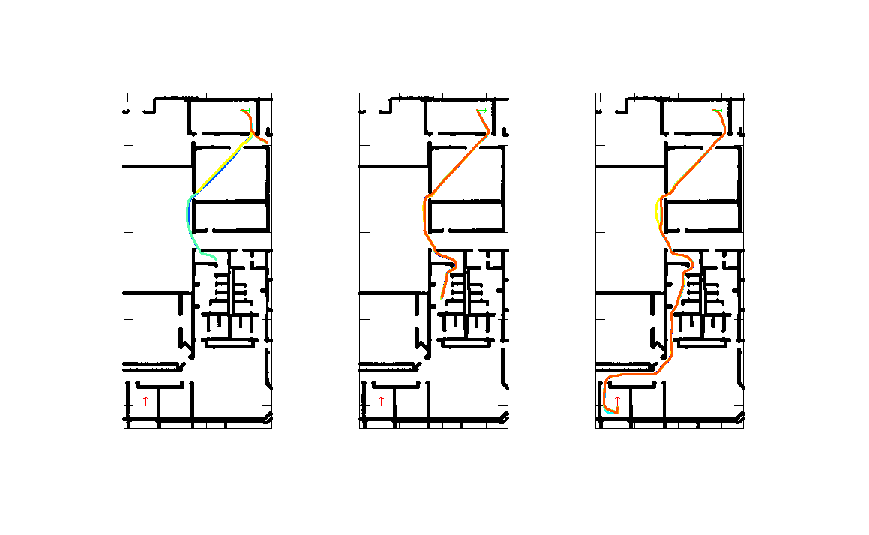
\includegraphics{./figures/parts/02/chapters/01/sections/04/ground_truth_sbpl_willowgarage}}%
    \gplfronttext
  \end{picture}%
\endgroup

  \end{subfigure}%
  \caption{\small Τα διανυθέντα μονοπάτια $\bm{\mathcal{P}}$ του ρομπότ, όπως
           ορίστηκαν από τους τρεις ελεγκτές κίνησης για κάθε συνδυασμό τους με
           αλγόριθμο παραγωγής μονοπατιών του πίνακα
           \ref{tbl:planners_sifted_list}, σε σχέση με τις ορισμένες αρχικές και
           τελικές στάσεις του περιβάλλοντος WILLOWGARAGE}
  \label{fig:ground_truths:willowgarage}
\end{figure}

Ο πίνακας \ref{tbl:rank_willowgarage} καταγράφει την τιμή-αξία $V_{\bm{M}_W}$
και την κατάταξη όλων των συνδυασμών αλγορίθμων χάραξης μονοπατιών και
ελεγκτών κίνησης που αξιολογήθηκαν με βάση τις τιμές όλων των μετρικών, που
παρουσιάζονται στους πίνακες \ref{tbl:info_global_plan_willowgarage}-
\ref{tbl:info_deviation_from_global_plan_willowgarage} όσον αφορά στις
επιδόσεις τους στην πλοήγηση στο περιβάλλον WILLOWGARAGE. Για τον υπολογισμό
της τιμής όλων των συνδυασμών, όλα τα βάρη $w_m = 1.0$ εκτός από αυτό που αφορά
στη μετρική $\mu_{PF} / \mu_{LPC}$, λόγω του γεγονότος ότι ότι ο
\texttt{eband\_local\_planner} δεν παρέχει πρόσβαση στον αριθμό των κλήσεων του
ελεγκτή. Συνολικά, ο ελεγκτής κίνησης \texttt{teb\_local\_planner} κατέλαβε και
πάλι όλες τις θέσεις του βάθρο (αυτή τη φορά λόγω της αποτυχίας όλων των άλλων
ελεγκτών κίνησης να ολοκληρώσουν την αποστολή του ρομπότ), με το συνδυασμό του
με τον \texttt{global\_planner} να ξεπερνά αυτόν με τον \texttt{navfn}, ο
οποίος ήταν ο συνολικά καλύτερος στο περιβάλλον CORRIDOR. Ενδιαφέρον αποτελεί
ότι ο \texttt{sbpl\_lattice\_planner} βοήθησε την επίδοση του
\texttt{dwa\_local\_planner} περισσότερο από τους άλλους global planners,
κάτι που πιθανότατα οφείλεται στο γεγονός ότι ο πρώτος λαμβάνει υπόψιν του
κατά την σχεδίαση των μονοπατιών τους περιορισμούς του κινηματικού μοντέλου
της βάσης του ρομπότ, το οποίο σε αυτήν την περίπτωση είναι διαφορικής κίνησης.


Λεπτομέρειες σχετικά με τις επιδόσεις των αλγορίθμων χάραξης μονοπατιών, των
ελεγκτών κίνησης, και των συνδυασμών τους, βρίσκονται στο παράρτημα
\ref{appendix:evaluation_willowgarage}.


\begin{table}[htb]\centering
\renewcommand{\arraystretch}{1.3}
\begin{tabular}{llccc}
  GP                     & LP             & επιτυχημένες αποστολές / $N$ & $V_{\bm{M}_W}$ & Κατάταξη \\ \toprule
  \texttt{globalplanner} & \texttt{teb}   & $10/10$                      & $21.90$        & $1$      \\
  \texttt{navfn}         & \texttt{teb}   & $10/10$                      & $20.00$        & $2$      \\
  \texttt{sbpl}          & \texttt{teb}   & $10/10$                      & $12.27$        & $3$      \\
  \texttt{globalplanner} & \texttt{eband} & $0/10$                       & $11.95$        & $4$      \\
  \texttt{navfn}         & \texttt{eband} & $0/10$                       & $11.76$        & $5$      \\
  \texttt{sbpl}          & \texttt{eband} & $0/10$                       & $9.85$         & $6$      \\
  \texttt{navfn}         & \texttt{dwa}   & $0/10$                       & $9.31$         & $7$      \\
  \texttt{globalplanner} & \texttt{dwa}   & $0/10$                       & $8.86$         & $8$      \\
  \texttt{sbpl}          & \texttt{dwa}   & $0/10$                       & $4.85$         & $9$      \\ \bottomrule
\end{tabular}
\caption{\small Οι αριθμοί επιτυχίας αποστολών, η τιμή-αξία $V_{\bm{M}_W}$, και
         η κατάταξη όλων των συνδυασμών των αλγορίθμων χάραξης μονοπατιών και
         ελεγκτών κίνησης που αξιολογούνται για τους την επίδοσή τους στο
         περιβάλλον WILLOWGARAGE σε $N=10$ προσομοιώσεις}
\label{tbl:rank_willowgarage}
\end{table}



%%%%%%%%%%%%%%%%%%%%%%%%%%%%%%%%%%%%%%%%%%%%%%%%%%%%%%%%%%%%%%%%%%%%%%%%%%%%%%%%
\subsection{Αξιολόγηση στο περιβάλλον CSAL}
  \label{subsection:02_01_04:04}

Συνολικά, όπως και στις προσομοιώσεις, όλοι οι συνδυασμοί αλγορίθμων
χάραξης μονοπατιών με τον ελεγκτή κίνησης \texttt{dwa\_local\_planner}
απέτυχαν να πλοηγήσουν το ρομπότ από την αρχική του στάση στην τελική. Οι
υπόλοιποι συνδυασμοί ήταν αξιόπιστοι σε κάθε εκτέλεση.

Το σχήμα \ref{fig:global_plans:csal} απεικονίζει τα μονοπάτια προς
ακολούθηση που παρήχθησαν από όλους τους global planners που εμφανίζονται στην
πρώτη στήλη του πίνακα \ref{tbl:planners_sifted_list}, για όλους τους
συνδυασμούς global και local planner του ίδιου πίνακα, για $N=10$ προσομοιώσεις
κάθε συνδυασμού.

\begin{figure*}
\raggedright
  \begin{subfigure}[t]{\linewidth}
    \centering
    % GNUPLOT: LaTeX picture with Postscript
\begingroup
  \makeatletter
  \providecommand\color[2][]{%
    \GenericError{(gnuplot) \space\space\space\@spaces}{%
      Package color not loaded in conjunction with
      terminal option `colourtext'%
    }{See the gnuplot documentation for explanation.%
    }{Either use 'blacktext' in gnuplot or load the package
      color.sty in LaTeX.}%
    \renewcommand\color[2][]{}%
  }%
  \providecommand\includegraphics[2][]{%
    \GenericError{(gnuplot) \space\space\space\@spaces}{%
      Package graphicx or graphics not loaded%
    }{See the gnuplot documentation for explanation.%
    }{The gnuplot epslatex terminal needs graphicx.sty or graphics.sty.}%
    \renewcommand\includegraphics[2][]{}%
  }%
  \providecommand\rotatebox[2]{#2}%
  \@ifundefined{ifGPcolor}{%
    \newif\ifGPcolor
    \GPcolorfalse
  }{}%
  \@ifundefined{ifGPblacktext}{%
    \newif\ifGPblacktext
    \GPblacktexttrue
  }{}%
  % define a \g@addto@macro without @ in the name:
  \let\gplgaddtomacro\g@addto@macro
  % define empty templates for all commands taking text:
  \gdef\gplfronttext{}%
  \gdef\gplfronttext{}%
  \makeatother
  \ifGPblacktext
    % no textcolor at all
    \def\colorrgb#1{}%
    \def\colorgray#1{}%
  \else
    % gray or color?
    \ifGPcolor
      \def\colorrgb#1{\color[rgb]{#1}}%
      \def\colorgray#1{\color[gray]{#1}}%
      \expandafter\def\csname LTw\endcsname{\color{white}}%
      \expandafter\def\csname LTb\endcsname{\color{black}}%
      \expandafter\def\csname LTa\endcsname{\color{black}}%
      \expandafter\def\csname LT0\endcsname{\color[rgb]{1,0,0}}%
      \expandafter\def\csname LT1\endcsname{\color[rgb]{0,1,0}}%
      \expandafter\def\csname LT2\endcsname{\color[rgb]{0,0,1}}%
      \expandafter\def\csname LT3\endcsname{\color[rgb]{1,0,1}}%
      \expandafter\def\csname LT4\endcsname{\color[rgb]{0,1,1}}%
      \expandafter\def\csname LT5\endcsname{\color[rgb]{1,1,0}}%
      \expandafter\def\csname LT6\endcsname{\color[rgb]{0,0,0}}%
      \expandafter\def\csname LT7\endcsname{\color[rgb]{1,0.3,0}}%
      \expandafter\def\csname LT8\endcsname{\color[rgb]{0.5,0.5,0.5}}%
    \else
      % gray
      \def\colorrgb#1{\color{black}}%
      \def\colorgray#1{\color[gray]{#1}}%
      \expandafter\def\csname LTw\endcsname{\color{white}}%
      \expandafter\def\csname LTb\endcsname{\color{black}}%
      \expandafter\def\csname LTa\endcsname{\color{black}}%
      \expandafter\def\csname LT0\endcsname{\color{black}}%
      \expandafter\def\csname LT1\endcsname{\color{black}}%
      \expandafter\def\csname LT2\endcsname{\color{black}}%
      \expandafter\def\csname LT3\endcsname{\color{black}}%
      \expandafter\def\csname LT4\endcsname{\color{black}}%
      \expandafter\def\csname LT5\endcsname{\color{black}}%
      \expandafter\def\csname LT6\endcsname{\color{black}}%
      \expandafter\def\csname LT7\endcsname{\color{black}}%
      \expandafter\def\csname LT8\endcsname{\color{black}}%
    \fi
  \fi
  \setlength{\unitlength}{0.0500bp}%
  \begin{picture}(10000.00,4000.00)%
    \gplgaddtomacro\gplfronttext{%
      \colorrgb{0.00,0.00,0.00}%
      \put(893,1120){\makebox(0,0)[r]{\strut{}$0$}}%
      \colorrgb{0.00,0.00,0.00}%
      \put(893,1657){\makebox(0,0)[r]{\strut{}$4$}}%
      \colorrgb{0.00,0.00,0.00}%
      \put(893,2194){\makebox(0,0)[r]{\strut{}$8$}}%
      \colorrgb{0.00,0.00,0.00}%
      \put(893,2731){\makebox(0,0)[r]{\strut{}$12$}}%
      \put(387,2059){\rotatebox{90}{\makebox(0,0){\strut{}$y$ [m]}}}%
      \colorrgb{0.00,0.00,0.00}%
      \put(2166,570){\makebox(0,0){\strut{}$x$ [m]}}%
      \colorrgb{0.00,0.00,0.00}%
      \put(2166,3329){\makebox(0,0){\strut{}\texttt{navfn} / \texttt{dwa}}}%
    }%
    \gplgaddtomacro\gplfronttext{%
    }%
    \gplgaddtomacro\gplfronttext{%
      \put(4999,3329){\makebox(0,0){\strut{}\texttt{navfn} / \texttt{eband}}}%
    }%
    \gplgaddtomacro\gplfronttext{%
    }%
    \gplgaddtomacro\gplfronttext{%
      \put(7832,3329){\makebox(0,0){\strut{}\texttt{navfn} / \texttt{teb}}}%
    }%
    \gplgaddtomacro\gplfronttext{%
    }%
    \put(0,0){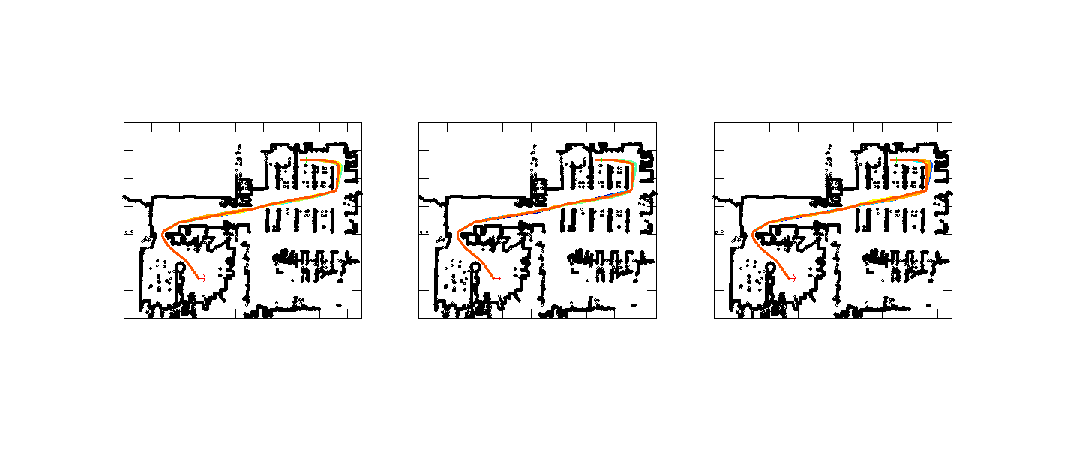
\includegraphics{./figures/parts/02/chapters/01/sections/04/global_plan_navfn_csal}}%
    \gplfronttext
  \end{picture}%
\endgroup

  \end{subfigure}%
  \vspace{-1.5cm}
  \begin{subfigure}[t]{\linewidth}
    \centering
    % GNUPLOT: LaTeX picture with Postscript
\begingroup
  \makeatletter
  \providecommand\color[2][]{%
    \GenericError{(gnuplot) \space\space\space\@spaces}{%
      Package color not loaded in conjunction with
      terminal option `colourtext'%
    }{See the gnuplot documentation for explanation.%
    }{Either use 'blacktext' in gnuplot or load the package
      color.sty in LaTeX.}%
    \renewcommand\color[2][]{}%
  }%
  \providecommand\includegraphics[2][]{%
    \GenericError{(gnuplot) \space\space\space\@spaces}{%
      Package graphicx or graphics not loaded%
    }{See the gnuplot documentation for explanation.%
    }{The gnuplot epslatex terminal needs graphicx.sty or graphics.sty.}%
    \renewcommand\includegraphics[2][]{}%
  }%
  \providecommand\rotatebox[2]{#2}%
  \@ifundefined{ifGPcolor}{%
    \newif\ifGPcolor
    \GPcolorfalse
  }{}%
  \@ifundefined{ifGPblacktext}{%
    \newif\ifGPblacktext
    \GPblacktexttrue
  }{}%
  % define a \g@addto@macro without @ in the name:
  \let\gplgaddtomacro\g@addto@macro
  % define empty templates for all commands taking text:
  \gdef\gplfronttext{}%
  \gdef\gplfronttext{}%
  \makeatother
  \ifGPblacktext
    % no textcolor at all
    \def\colorrgb#1{}%
    \def\colorgray#1{}%
  \else
    % gray or color?
    \ifGPcolor
      \def\colorrgb#1{\color[rgb]{#1}}%
      \def\colorgray#1{\color[gray]{#1}}%
      \expandafter\def\csname LTw\endcsname{\color{white}}%
      \expandafter\def\csname LTb\endcsname{\color{black}}%
      \expandafter\def\csname LTa\endcsname{\color{black}}%
      \expandafter\def\csname LT0\endcsname{\color[rgb]{1,0,0}}%
      \expandafter\def\csname LT1\endcsname{\color[rgb]{0,1,0}}%
      \expandafter\def\csname LT2\endcsname{\color[rgb]{0,0,1}}%
      \expandafter\def\csname LT3\endcsname{\color[rgb]{1,0,1}}%
      \expandafter\def\csname LT4\endcsname{\color[rgb]{0,1,1}}%
      \expandafter\def\csname LT5\endcsname{\color[rgb]{1,1,0}}%
      \expandafter\def\csname LT6\endcsname{\color[rgb]{0,0,0}}%
      \expandafter\def\csname LT7\endcsname{\color[rgb]{1,0.3,0}}%
      \expandafter\def\csname LT8\endcsname{\color[rgb]{0.5,0.5,0.5}}%
    \else
      % gray
      \def\colorrgb#1{\color{black}}%
      \def\colorgray#1{\color[gray]{#1}}%
      \expandafter\def\csname LTw\endcsname{\color{white}}%
      \expandafter\def\csname LTb\endcsname{\color{black}}%
      \expandafter\def\csname LTa\endcsname{\color{black}}%
      \expandafter\def\csname LT0\endcsname{\color{black}}%
      \expandafter\def\csname LT1\endcsname{\color{black}}%
      \expandafter\def\csname LT2\endcsname{\color{black}}%
      \expandafter\def\csname LT3\endcsname{\color{black}}%
      \expandafter\def\csname LT4\endcsname{\color{black}}%
      \expandafter\def\csname LT5\endcsname{\color{black}}%
      \expandafter\def\csname LT6\endcsname{\color{black}}%
      \expandafter\def\csname LT7\endcsname{\color{black}}%
      \expandafter\def\csname LT8\endcsname{\color{black}}%
    \fi
  \fi
  \setlength{\unitlength}{0.0500bp}%
  \begin{picture}(10000.00,4000.00)%
    \gplgaddtomacro\gplfronttext{%
      \colorrgb{0.00,0.00,0.00}%
      \put(893,1120){\makebox(0,0)[r]{\strut{}$0$}}%
      \colorrgb{0.00,0.00,0.00}%
      \put(893,1657){\makebox(0,0)[r]{\strut{}$4$}}%
      \colorrgb{0.00,0.00,0.00}%
      \put(893,2194){\makebox(0,0)[r]{\strut{}$8$}}%
      \colorrgb{0.00,0.00,0.00}%
      \put(893,2731){\makebox(0,0)[r]{\strut{}$12$}}%
      \put(387,2059){\rotatebox{90}{\makebox(0,0){\strut{}$y$ [m]}}}%
      \put(2166,3329){\makebox(0,0){\strut{}\texttt{global\_planner} / \texttt{dwa}}}%
    }%
    \gplgaddtomacro\gplfronttext{%
    }%
    \gplgaddtomacro\gplfronttext{%
      \put(4999,3329){\makebox(0,0){\strut{}\texttt{global\_planner} / \texttt{eband}}}%
    }%
    \gplgaddtomacro\gplfronttext{%
    }%
    \gplgaddtomacro\gplfronttext{%
      \put(7832,3329){\makebox(0,0){\strut{}\texttt{global\_planner} / \texttt{teb}}}%
    }%
    \gplgaddtomacro\gplfronttext{%
    }%
    \put(0,0){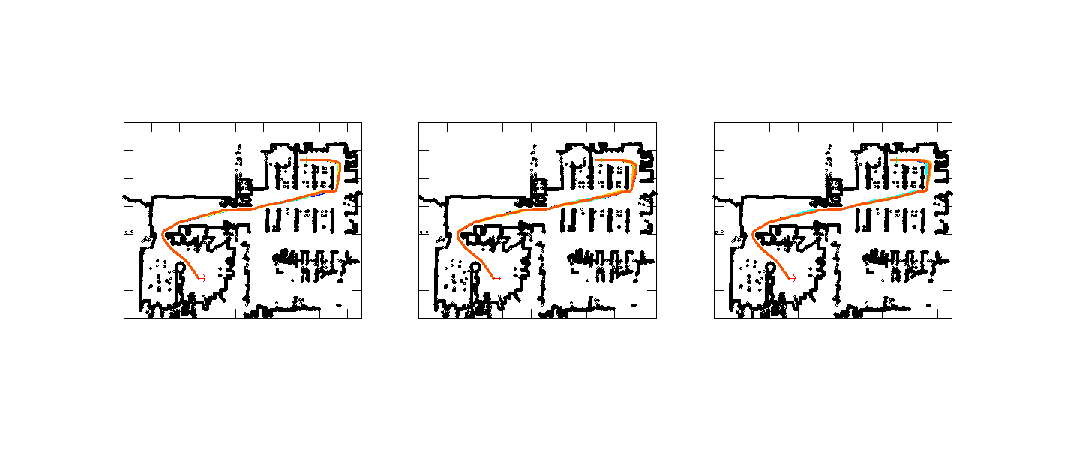
\includegraphics{./figures/parts/02/chapters/01/sections/04/global_plan_globalplanner_csal}}%
    \gplfronttext
  \end{picture}%
\endgroup

  \end{subfigure}%
  \vspace{-1.5cm}
  \begin{subfigure}[t]{\linewidth}
    \centering
    % GNUPLOT: LaTeX picture with Postscript
\begingroup
  \makeatletter
  \providecommand\color[2][]{%
    \GenericError{(gnuplot) \space\space\space\@spaces}{%
      Package color not loaded in conjunction with
      terminal option `colourtext'%
    }{See the gnuplot documentation for explanation.%
    }{Either use 'blacktext' in gnuplot or load the package
      color.sty in LaTeX.}%
    \renewcommand\color[2][]{}%
  }%
  \providecommand\includegraphics[2][]{%
    \GenericError{(gnuplot) \space\space\space\@spaces}{%
      Package graphicx or graphics not loaded%
    }{See the gnuplot documentation for explanation.%
    }{The gnuplot epslatex terminal needs graphicx.sty or graphics.sty.}%
    \renewcommand\includegraphics[2][]{}%
  }%
  \providecommand\rotatebox[2]{#2}%
  \@ifundefined{ifGPcolor}{%
    \newif\ifGPcolor
    \GPcolorfalse
  }{}%
  \@ifundefined{ifGPblacktext}{%
    \newif\ifGPblacktext
    \GPblacktexttrue
  }{}%
  % define a \g@addto@macro without @ in the name:
  \let\gplgaddtomacro\g@addto@macro
  % define empty templates for all commands taking text:
  \gdef\gplfronttext{}%
  \gdef\gplfronttext{}%
  \makeatother
  \ifGPblacktext
    % no textcolor at all
    \def\colorrgb#1{}%
    \def\colorgray#1{}%
  \else
    % gray or color?
    \ifGPcolor
      \def\colorrgb#1{\color[rgb]{#1}}%
      \def\colorgray#1{\color[gray]{#1}}%
      \expandafter\def\csname LTw\endcsname{\color{white}}%
      \expandafter\def\csname LTb\endcsname{\color{black}}%
      \expandafter\def\csname LTa\endcsname{\color{black}}%
      \expandafter\def\csname LT0\endcsname{\color[rgb]{1,0,0}}%
      \expandafter\def\csname LT1\endcsname{\color[rgb]{0,1,0}}%
      \expandafter\def\csname LT2\endcsname{\color[rgb]{0,0,1}}%
      \expandafter\def\csname LT3\endcsname{\color[rgb]{1,0,1}}%
      \expandafter\def\csname LT4\endcsname{\color[rgb]{0,1,1}}%
      \expandafter\def\csname LT5\endcsname{\color[rgb]{1,1,0}}%
      \expandafter\def\csname LT6\endcsname{\color[rgb]{0,0,0}}%
      \expandafter\def\csname LT7\endcsname{\color[rgb]{1,0.3,0}}%
      \expandafter\def\csname LT8\endcsname{\color[rgb]{0.5,0.5,0.5}}%
    \else
      % gray
      \def\colorrgb#1{\color{black}}%
      \def\colorgray#1{\color[gray]{#1}}%
      \expandafter\def\csname LTw\endcsname{\color{white}}%
      \expandafter\def\csname LTb\endcsname{\color{black}}%
      \expandafter\def\csname LTa\endcsname{\color{black}}%
      \expandafter\def\csname LT0\endcsname{\color{black}}%
      \expandafter\def\csname LT1\endcsname{\color{black}}%
      \expandafter\def\csname LT2\endcsname{\color{black}}%
      \expandafter\def\csname LT3\endcsname{\color{black}}%
      \expandafter\def\csname LT4\endcsname{\color{black}}%
      \expandafter\def\csname LT5\endcsname{\color{black}}%
      \expandafter\def\csname LT6\endcsname{\color{black}}%
      \expandafter\def\csname LT7\endcsname{\color{black}}%
      \expandafter\def\csname LT8\endcsname{\color{black}}%
    \fi
  \fi
  \setlength{\unitlength}{0.0500bp}%
  \begin{picture}(10000.00,4000.00)%
    \gplgaddtomacro\gplfronttext{%
      \colorrgb{0.00,0.00,0.00}%
      \put(893,1120){\makebox(0,0)[r]{\strut{}$0$}}%
      \colorrgb{0.00,0.00,0.00}%
      \put(893,1657){\makebox(0,0)[r]{\strut{}$4$}}%
      \colorrgb{0.00,0.00,0.00}%
      \put(893,2194){\makebox(0,0)[r]{\strut{}$8$}}%
      \colorrgb{0.00,0.00,0.00}%
      \put(893,2731){\makebox(0,0)[r]{\strut{}$12$}}%
      \colorrgb{0.00,0.00,0.00}%
      \put(1025,900){\makebox(0,0){\strut{}$6$}}%
      \colorrgb{0.00,0.00,0.00}%
      \put(1562,900){\makebox(0,0){\strut{}$10$}}%
      \colorrgb{0.00,0.00,0.00}%
      \put(2099,900){\makebox(0,0){\strut{}$14$}}%
      \colorrgb{0.00,0.00,0.00}%
      \put(2636,900){\makebox(0,0){\strut{}$18$}}%
      \colorrgb{0.00,0.00,0.00}%
      \put(3173,900){\makebox(0,0){\strut{}$22$}}%
      \colorrgb{0.00,0.00,0.00}%
      \put(387,2059){\rotatebox{90}{\makebox(0,0){\strut{}$y$ [m]}}}%
      \colorrgb{0.00,0.00,0.00}%
      \put(2166,570){\makebox(0,0){\strut{}$x$ [m]}}%
      \colorrgb{0.00,0.00,0.00}%
      \put(2166,3329){\makebox(0,0){\strut{}\texttt{sbpl} / \texttt{dwa}}}%
    }%
    \gplgaddtomacro\gplfronttext{%
    }%
    \gplgaddtomacro\gplfronttext{%
      \put(3858,900){\makebox(0,0){\strut{}$6$}}%
      \colorrgb{0.00,0.00,0.00}%
      \put(4395,900){\makebox(0,0){\strut{}$10$}}%
      \colorrgb{0.00,0.00,0.00}%
      \put(4932,900){\makebox(0,0){\strut{}$14$}}%
      \colorrgb{0.00,0.00,0.00}%
      \put(5469,900){\makebox(0,0){\strut{}$18$}}%
      \colorrgb{0.00,0.00,0.00}%
      \put(6006,900){\makebox(0,0){\strut{}$22$}}%
      \colorrgb{0.00,0.00,0.00}%
      \put(4999,570){\makebox(0,0){\strut{}$x$ [m]}}%
      \colorrgb{0.00,0.00,0.00}%
      \put(4999,3329){\makebox(0,0){\strut{}\texttt{sbpl} / \texttt{eband}}}%
    }%
    \gplgaddtomacro\gplfronttext{%
    }%
    \gplgaddtomacro\gplfronttext{%
      \put(6691,900){\makebox(0,0){\strut{}$6$}}%
      \colorrgb{0.00,0.00,0.00}%
      \put(7228,900){\makebox(0,0){\strut{}$10$}}%
      \colorrgb{0.00,0.00,0.00}%
      \put(7765,900){\makebox(0,0){\strut{}$14$}}%
      \colorrgb{0.00,0.00,0.00}%
      \put(8302,900){\makebox(0,0){\strut{}$18$}}%
      \colorrgb{0.00,0.00,0.00}%
      \put(8839,900){\makebox(0,0){\strut{}$22$}}%
      \colorrgb{0.00,0.00,0.00}%
      \put(7832,570){\makebox(0,0){\strut{}$x$ [m]}}%
      \colorrgb{0.00,0.00,0.00}%
      \put(7832,3329){\makebox(0,0){\strut{}\texttt{sbpl} / \texttt{teb}}}%
    }%
    \gplgaddtomacro\gplfronttext{%
    }%
    \put(0,0){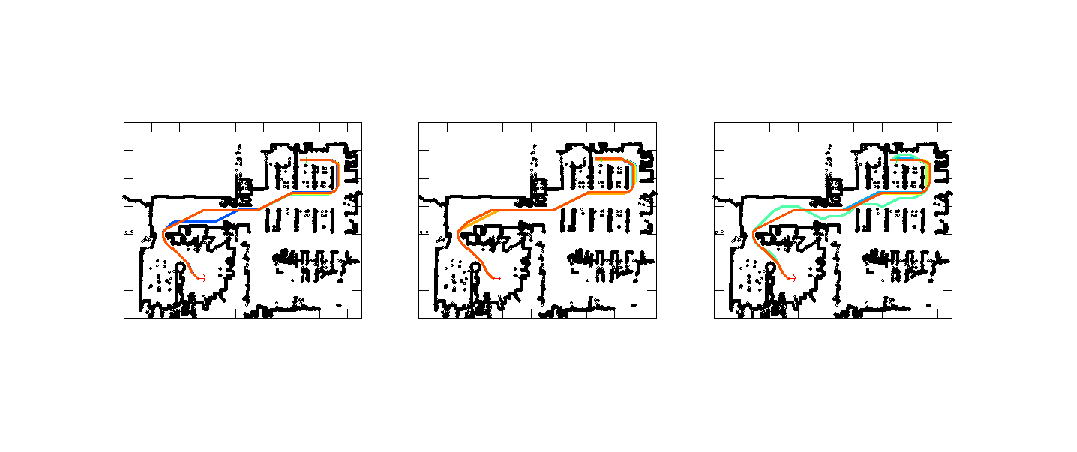
\includegraphics{./figures/parts/02/chapters/01/sections/04/global_plan_sbpl_csal}}%
    \gplfronttext
  \end{picture}%
\endgroup

  \end{subfigure}%
  \caption{\small Τα σχεδιασθέντα μονοπάτια προς ακολούθηση $\bm{\mathcal{G}}$
           που παρήχθησαν από τους τρεις αλγορίθμους χάραξης μονοπατιών για
           κάθε συνδυασμό τους με ελεγκτή κίνησης του πίνακα
           \ref{tbl:planners_sifted_list}, σε σχέση με τις ορισμένες αρχικές και
           τελικές στάσεις του περιβάλλοντος CSAL}
  \label{fig:global_plans:csal}
\end{figure*}

Το σχήμα \ref{fig:poses:csal} απεικονίζει τις εκτιμώμενες \footnote{Το
εργαστήριο CSAL, σε αντίθεση με το περιβάλλον προσομοίωσης Gazebo, δεν διαθέτει
υποδομή μέτρησης της πραγματικής στάσης ενός οχήματος. Oι εκτιμώμενες διαδρομές
βασίζονται στην εκτίμησης της στάσης του ρομπότ, η οποία εξάγεται μέσω της
χρήσης φίλτρου σωματιδίου. Η λειτουργία του φίλτρου βασίζεται στο κινηματικό
μοντέλο της βάσης του Turtlebot, η οποία είναι διαφορικής φύσης, και σε έναν
αισθητήρα αποστάσεων 2D lidar.} διαδρομές που διένυσε το ρομπότ για όλους τους
συνδυασμούς αλγορίθμων σχεδίασης μονοπατιών και ελεγκτών κίνησης του ίδιου
πίνακα, για $N=10$ προσομοιώσεις για κάθε συνδυασμό.

\begin{figure*}\centering
  \begin{subfigure}[t]{\linewidth}
    \centering
    % GNUPLOT: LaTeX picture with Postscript
\begingroup
  \makeatletter
  \providecommand\color[2][]{%
    \GenericError{(gnuplot) \space\space\space\@spaces}{%
      Package color not loaded in conjunction with
      terminal option `colourtext'%
    }{See the gnuplot documentation for explanation.%
    }{Either use 'blacktext' in gnuplot or load the package
      color.sty in LaTeX.}%
    \renewcommand\color[2][]{}%
  }%
  \providecommand\includegraphics[2][]{%
    \GenericError{(gnuplot) \space\space\space\@spaces}{%
      Package graphicx or graphics not loaded%
    }{See the gnuplot documentation for explanation.%
    }{The gnuplot epslatex terminal needs graphicx.sty or graphics.sty.}%
    \renewcommand\includegraphics[2][]{}%
  }%
  \providecommand\rotatebox[2]{#2}%
  \@ifundefined{ifGPcolor}{%
    \newif\ifGPcolor
    \GPcolorfalse
  }{}%
  \@ifundefined{ifGPblacktext}{%
    \newif\ifGPblacktext
    \GPblacktexttrue
  }{}%
  % define a \g@addto@macro without @ in the name:
  \let\gplgaddtomacro\g@addto@macro
  % define empty templates for all commands taking text:
  \gdef\gplfronttext{}%
  \gdef\gplfronttext{}%
  \makeatother
  \ifGPblacktext
    % no textcolor at all
    \def\colorrgb#1{}%
    \def\colorgray#1{}%
  \else
    % gray or color?
    \ifGPcolor
      \def\colorrgb#1{\color[rgb]{#1}}%
      \def\colorgray#1{\color[gray]{#1}}%
      \expandafter\def\csname LTw\endcsname{\color{white}}%
      \expandafter\def\csname LTb\endcsname{\color{black}}%
      \expandafter\def\csname LTa\endcsname{\color{black}}%
      \expandafter\def\csname LT0\endcsname{\color[rgb]{1,0,0}}%
      \expandafter\def\csname LT1\endcsname{\color[rgb]{0,1,0}}%
      \expandafter\def\csname LT2\endcsname{\color[rgb]{0,0,1}}%
      \expandafter\def\csname LT3\endcsname{\color[rgb]{1,0,1}}%
      \expandafter\def\csname LT4\endcsname{\color[rgb]{0,1,1}}%
      \expandafter\def\csname LT5\endcsname{\color[rgb]{1,1,0}}%
      \expandafter\def\csname LT6\endcsname{\color[rgb]{0,0,0}}%
      \expandafter\def\csname LT7\endcsname{\color[rgb]{1,0.3,0}}%
      \expandafter\def\csname LT8\endcsname{\color[rgb]{0.5,0.5,0.5}}%
    \else
      % gray
      \def\colorrgb#1{\color{black}}%
      \def\colorgray#1{\color[gray]{#1}}%
      \expandafter\def\csname LTw\endcsname{\color{white}}%
      \expandafter\def\csname LTb\endcsname{\color{black}}%
      \expandafter\def\csname LTa\endcsname{\color{black}}%
      \expandafter\def\csname LT0\endcsname{\color{black}}%
      \expandafter\def\csname LT1\endcsname{\color{black}}%
      \expandafter\def\csname LT2\endcsname{\color{black}}%
      \expandafter\def\csname LT3\endcsname{\color{black}}%
      \expandafter\def\csname LT4\endcsname{\color{black}}%
      \expandafter\def\csname LT5\endcsname{\color{black}}%
      \expandafter\def\csname LT6\endcsname{\color{black}}%
      \expandafter\def\csname LT7\endcsname{\color{black}}%
      \expandafter\def\csname LT8\endcsname{\color{black}}%
    \fi
  \fi
  \setlength{\unitlength}{0.0500bp}%
  \begin{picture}(10000.00,4000.00)%
    \gplgaddtomacro\gplfronttext{%
      \colorrgb{0.00,0.00,0.00}%
      \put(893,1120){\makebox(0,0)[r]{\strut{}$0$}}%
      \colorrgb{0.00,0.00,0.00}%
      \put(893,1657){\makebox(0,0)[r]{\strut{}$4$}}%
      \colorrgb{0.00,0.00,0.00}%
      \put(893,2194){\makebox(0,0)[r]{\strut{}$8$}}%
      \colorrgb{0.00,0.00,0.00}%
      \put(893,2731){\makebox(0,0)[r]{\strut{}$12$}}%
      \put(387,2059){\rotatebox{90}{\makebox(0,0){\strut{}$y$ [m]}}}%
      \colorrgb{0.00,0.00,0.00}%
      \put(2166,570){\makebox(0,0){\strut{}$x$ [m]}}%
      \colorrgb{0.00,0.00,0.00}%
      \put(2166,3279){\makebox(0,0){\strut{}\texttt{navfn}/\texttt{dwa}}}%
    }%
    \gplgaddtomacro\gplfronttext{%
    }%
    \gplgaddtomacro\gplfronttext{%
      \put(4999,3279){\makebox(0,0){\strut{}\texttt{navfn}/\texttt{eband}}}%
    }%
    \gplgaddtomacro\gplfronttext{%
    }%
    \gplgaddtomacro\gplfronttext{%
      \put(7832,3279){\makebox(0,0){\strut{}\texttt{navfn}/\texttt{teb}}}%
    }%
    \gplgaddtomacro\gplfronttext{%
    }%
    \put(0,0){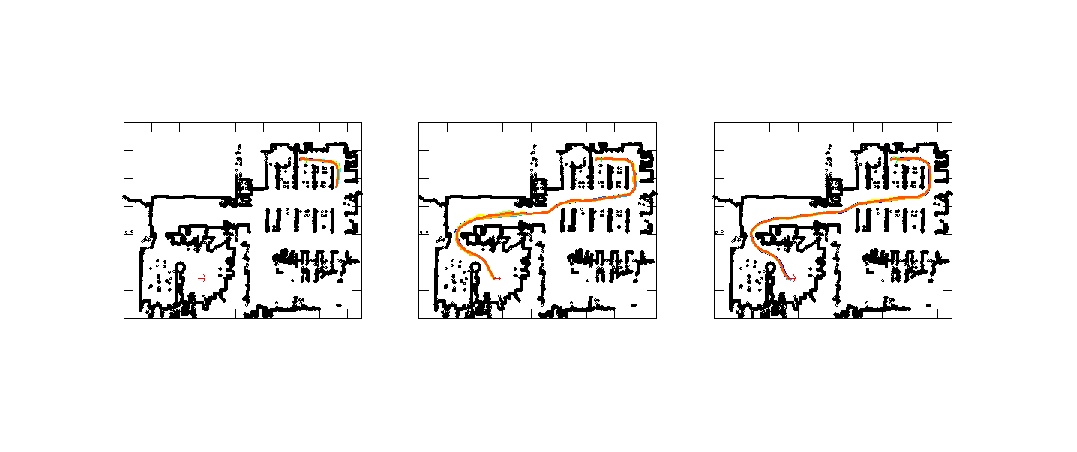
\includegraphics{./figures/parts/02/chapters/01/sections/04/pose_navfn_csal}}%
    \gplfronttext
  \end{picture}%
\endgroup

  \end{subfigure}\\%
  \vspace{-1.5cm}
  \begin{subfigure}[t]{\linewidth}
    \centering
    % GNUPLOT: LaTeX picture with Postscript
\begingroup
  \makeatletter
  \providecommand\color[2][]{%
    \GenericError{(gnuplot) \space\space\space\@spaces}{%
      Package color not loaded in conjunction with
      terminal option `colourtext'%
    }{See the gnuplot documentation for explanation.%
    }{Either use 'blacktext' in gnuplot or load the package
      color.sty in LaTeX.}%
    \renewcommand\color[2][]{}%
  }%
  \providecommand\includegraphics[2][]{%
    \GenericError{(gnuplot) \space\space\space\@spaces}{%
      Package graphicx or graphics not loaded%
    }{See the gnuplot documentation for explanation.%
    }{The gnuplot epslatex terminal needs graphicx.sty or graphics.sty.}%
    \renewcommand\includegraphics[2][]{}%
  }%
  \providecommand\rotatebox[2]{#2}%
  \@ifundefined{ifGPcolor}{%
    \newif\ifGPcolor
    \GPcolorfalse
  }{}%
  \@ifundefined{ifGPblacktext}{%
    \newif\ifGPblacktext
    \GPblacktexttrue
  }{}%
  % define a \g@addto@macro without @ in the name:
  \let\gplgaddtomacro\g@addto@macro
  % define empty templates for all commands taking text:
  \gdef\gplfronttext{}%
  \gdef\gplfronttext{}%
  \makeatother
  \ifGPblacktext
    % no textcolor at all
    \def\colorrgb#1{}%
    \def\colorgray#1{}%
  \else
    % gray or color?
    \ifGPcolor
      \def\colorrgb#1{\color[rgb]{#1}}%
      \def\colorgray#1{\color[gray]{#1}}%
      \expandafter\def\csname LTw\endcsname{\color{white}}%
      \expandafter\def\csname LTb\endcsname{\color{black}}%
      \expandafter\def\csname LTa\endcsname{\color{black}}%
      \expandafter\def\csname LT0\endcsname{\color[rgb]{1,0,0}}%
      \expandafter\def\csname LT1\endcsname{\color[rgb]{0,1,0}}%
      \expandafter\def\csname LT2\endcsname{\color[rgb]{0,0,1}}%
      \expandafter\def\csname LT3\endcsname{\color[rgb]{1,0,1}}%
      \expandafter\def\csname LT4\endcsname{\color[rgb]{0,1,1}}%
      \expandafter\def\csname LT5\endcsname{\color[rgb]{1,1,0}}%
      \expandafter\def\csname LT6\endcsname{\color[rgb]{0,0,0}}%
      \expandafter\def\csname LT7\endcsname{\color[rgb]{1,0.3,0}}%
      \expandafter\def\csname LT8\endcsname{\color[rgb]{0.5,0.5,0.5}}%
    \else
      % gray
      \def\colorrgb#1{\color{black}}%
      \def\colorgray#1{\color[gray]{#1}}%
      \expandafter\def\csname LTw\endcsname{\color{white}}%
      \expandafter\def\csname LTb\endcsname{\color{black}}%
      \expandafter\def\csname LTa\endcsname{\color{black}}%
      \expandafter\def\csname LT0\endcsname{\color{black}}%
      \expandafter\def\csname LT1\endcsname{\color{black}}%
      \expandafter\def\csname LT2\endcsname{\color{black}}%
      \expandafter\def\csname LT3\endcsname{\color{black}}%
      \expandafter\def\csname LT4\endcsname{\color{black}}%
      \expandafter\def\csname LT5\endcsname{\color{black}}%
      \expandafter\def\csname LT6\endcsname{\color{black}}%
      \expandafter\def\csname LT7\endcsname{\color{black}}%
      \expandafter\def\csname LT8\endcsname{\color{black}}%
    \fi
  \fi
  \setlength{\unitlength}{0.0500bp}%
  \begin{picture}(10000.00,4000.00)%
    \gplgaddtomacro\gplfronttext{%
      \colorrgb{0.00,0.00,0.00}%
      \put(893,1120){\makebox(0,0)[r]{\strut{}$0$}}%
      \colorrgb{0.00,0.00,0.00}%
      \put(893,1657){\makebox(0,0)[r]{\strut{}$4$}}%
      \colorrgb{0.00,0.00,0.00}%
      \put(893,2194){\makebox(0,0)[r]{\strut{}$8$}}%
      \colorrgb{0.00,0.00,0.00}%
      \put(893,2731){\makebox(0,0)[r]{\strut{}$12$}}%
      \put(387,2059){\rotatebox{90}{\makebox(0,0){\strut{}$y$ [m]}}}%
      \colorrgb{0.00,0.00,0.00}%
      \put(2166,570){\makebox(0,0){\strut{}$x$ [m]}}%
      \colorrgb{0.00,0.00,0.00}%
      \put(2166,3329){\makebox(0,0){\strut{}\texttt{global\_planner} / \texttt{dwa}}}%
    }%
    \gplgaddtomacro\gplfronttext{%
    }%
    \gplgaddtomacro\gplfronttext{%
      \put(4999,3329){\makebox(0,0){\strut{}\texttt{global\_planner} / \texttt{eband}}}%
    }%
    \gplgaddtomacro\gplfronttext{%
    }%
    \gplgaddtomacro\gplfronttext{%
      \put(7832,570){\makebox(0,0){\strut{}$x$ [m]}}%
      \colorrgb{0.00,0.00,0.00}%
      \put(7832,3329){\makebox(0,0){\strut{}\texttt{global\_planner} / \texttt{teb}}}%
    }%
    \gplgaddtomacro\gplfronttext{%
    }%
    \gplfronttext
    \put(0,0){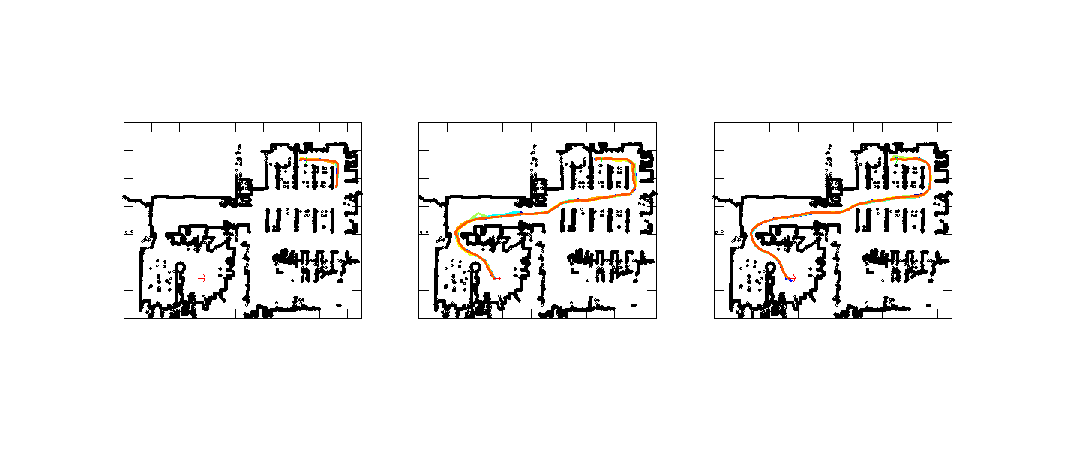
\includegraphics{./figures/parts/02/chapters/01/sections/04/pose_globalplanner_csal}}%
    \gplfronttext
  \end{picture}%
\endgroup

  \end{subfigure}\\%
  \vspace{-1.5cm}
  \begin{subfigure}[t]{\linewidth}
    \centering
    % GNUPLOT: LaTeX picture with Postscript
\begingroup
  \makeatletter
  \providecommand\color[2][]{%
    \GenericError{(gnuplot) \space\space\space\@spaces}{%
      Package color not loaded in conjunction with
      terminal option `colourtext'%
    }{See the gnuplot documentation for explanation.%
    }{Either use 'blacktext' in gnuplot or load the package
      color.sty in LaTeX.}%
    \renewcommand\color[2][]{}%
  }%
  \providecommand\includegraphics[2][]{%
    \GenericError{(gnuplot) \space\space\space\@spaces}{%
      Package graphicx or graphics not loaded%
    }{See the gnuplot documentation for explanation.%
    }{The gnuplot epslatex terminal needs graphicx.sty or graphics.sty.}%
    \renewcommand\includegraphics[2][]{}%
  }%
  \providecommand\rotatebox[2]{#2}%
  \@ifundefined{ifGPcolor}{%
    \newif\ifGPcolor
    \GPcolorfalse
  }{}%
  \@ifundefined{ifGPblacktext}{%
    \newif\ifGPblacktext
    \GPblacktexttrue
  }{}%
  % define a \g@addto@macro without @ in the name:
  \let\gplgaddtomacro\g@addto@macro
  % define empty templates for all commands taking text:
  \gdef\gplfronttext{}%
  \gdef\gplfronttext{}%
  \makeatother
  \ifGPblacktext
    % no textcolor at all
    \def\colorrgb#1{}%
    \def\colorgray#1{}%
  \else
    % gray or color?
    \ifGPcolor
      \def\colorrgb#1{\color[rgb]{#1}}%
      \def\colorgray#1{\color[gray]{#1}}%
      \expandafter\def\csname LTw\endcsname{\color{white}}%
      \expandafter\def\csname LTb\endcsname{\color{black}}%
      \expandafter\def\csname LTa\endcsname{\color{black}}%
      \expandafter\def\csname LT0\endcsname{\color[rgb]{1,0,0}}%
      \expandafter\def\csname LT1\endcsname{\color[rgb]{0,1,0}}%
      \expandafter\def\csname LT2\endcsname{\color[rgb]{0,0,1}}%
      \expandafter\def\csname LT3\endcsname{\color[rgb]{1,0,1}}%
      \expandafter\def\csname LT4\endcsname{\color[rgb]{0,1,1}}%
      \expandafter\def\csname LT5\endcsname{\color[rgb]{1,1,0}}%
      \expandafter\def\csname LT6\endcsname{\color[rgb]{0,0,0}}%
      \expandafter\def\csname LT7\endcsname{\color[rgb]{1,0.3,0}}%
      \expandafter\def\csname LT8\endcsname{\color[rgb]{0.5,0.5,0.5}}%
    \else
      % gray
      \def\colorrgb#1{\color{black}}%
      \def\colorgray#1{\color[gray]{#1}}%
      \expandafter\def\csname LTw\endcsname{\color{white}}%
      \expandafter\def\csname LTb\endcsname{\color{black}}%
      \expandafter\def\csname LTa\endcsname{\color{black}}%
      \expandafter\def\csname LT0\endcsname{\color{black}}%
      \expandafter\def\csname LT1\endcsname{\color{black}}%
      \expandafter\def\csname LT2\endcsname{\color{black}}%
      \expandafter\def\csname LT3\endcsname{\color{black}}%
      \expandafter\def\csname LT4\endcsname{\color{black}}%
      \expandafter\def\csname LT5\endcsname{\color{black}}%
      \expandafter\def\csname LT6\endcsname{\color{black}}%
      \expandafter\def\csname LT7\endcsname{\color{black}}%
      \expandafter\def\csname LT8\endcsname{\color{black}}%
    \fi
  \fi
  \setlength{\unitlength}{0.0500bp}%
  \begin{picture}(10000.00,4000.00)%
    \gplgaddtomacro\gplfronttext{%
      \colorrgb{0.00,0.00,0.00}%
      \put(893,1120){\makebox(0,0)[r]{\strut{}$0$}}%
      \colorrgb{0.00,0.00,0.00}%
      \put(893,1657){\makebox(0,0)[r]{\strut{}$4$}}%
      \colorrgb{0.00,0.00,0.00}%
      \put(893,2194){\makebox(0,0)[r]{\strut{}$8$}}%
      \colorrgb{0.00,0.00,0.00}%
      \put(893,2731){\makebox(0,0)[r]{\strut{}$12$}}%
      \colorrgb{0.00,0.00,0.00}%
      \put(1025,900){\makebox(0,0){\strut{}$6$}}%
      \colorrgb{0.00,0.00,0.00}%
      \put(1562,900){\makebox(0,0){\strut{}$10$}}%
      \colorrgb{0.00,0.00,0.00}%
      \put(2099,900){\makebox(0,0){\strut{}$14$}}%
      \colorrgb{0.00,0.00,0.00}%
      \put(2636,900){\makebox(0,0){\strut{}$18$}}%
      \colorrgb{0.00,0.00,0.00}%
      \put(3173,900){\makebox(0,0){\strut{}$22$}}%
      \colorrgb{0.00,0.00,0.00}%
      \put(387,2059){\rotatebox{90}{\makebox(0,0){\strut{}$y$ [m]}}}%
      \colorrgb{0.00,0.00,0.00}%
      \put(2166,570){\makebox(0,0){\strut{}$x$ [m]}}%
      \colorrgb{0.00,0.00,0.00}%
      \put(2166,3329){\makebox(0,0){\strut{}\texttt{sbpl} / \texttt{dwa}}}%
    }%
    \gplgaddtomacro\gplfronttext{%
    }%
    \gplgaddtomacro\gplfronttext{%
      \put(3858,900){\makebox(0,0){\strut{}$6$}}%
      \colorrgb{0.00,0.00,0.00}%
      \put(4395,900){\makebox(0,0){\strut{}$10$}}%
      \colorrgb{0.00,0.00,0.00}%
      \put(4932,900){\makebox(0,0){\strut{}$14$}}%
      \colorrgb{0.00,0.00,0.00}%
      \put(5469,900){\makebox(0,0){\strut{}$18$}}%
      \colorrgb{0.00,0.00,0.00}%
      \put(6006,900){\makebox(0,0){\strut{}$22$}}%
      \colorrgb{0.00,0.00,0.00}%
      \put(4999,570){\makebox(0,0){\strut{}$x$ [m]}}%
      \colorrgb{0.00,0.00,0.00}%
      \put(4999,3329){\makebox(0,0){\strut{}\texttt{sbpl} / \texttt{eband}}}%
    }%
    \gplgaddtomacro\gplfronttext{%
    }%
    \gplgaddtomacro\gplfronttext{%
      \put(6691,900){\makebox(0,0){\strut{}$6$}}%
      \colorrgb{0.00,0.00,0.00}%
      \put(7228,900){\makebox(0,0){\strut{}$10$}}%
      \colorrgb{0.00,0.00,0.00}%
      \put(7765,900){\makebox(0,0){\strut{}$14$}}%
      \colorrgb{0.00,0.00,0.00}%
      \put(8302,900){\makebox(0,0){\strut{}$18$}}%
      \colorrgb{0.00,0.00,0.00}%
      \put(8839,900){\makebox(0,0){\strut{}$22$}}%
      \colorrgb{0.00,0.00,0.00}%
      \put(7832,570){\makebox(0,0){\strut{}$x$ [m]}}%
      \colorrgb{0.00,0.00,0.00}%
      \put(7832,3329){\makebox(0,0){\strut{}\texttt{sbpl} / \texttt{teb}}}%
    }%
    \gplgaddtomacro\gplfronttext{%
    }%
    \gplfronttext
    \put(0,0){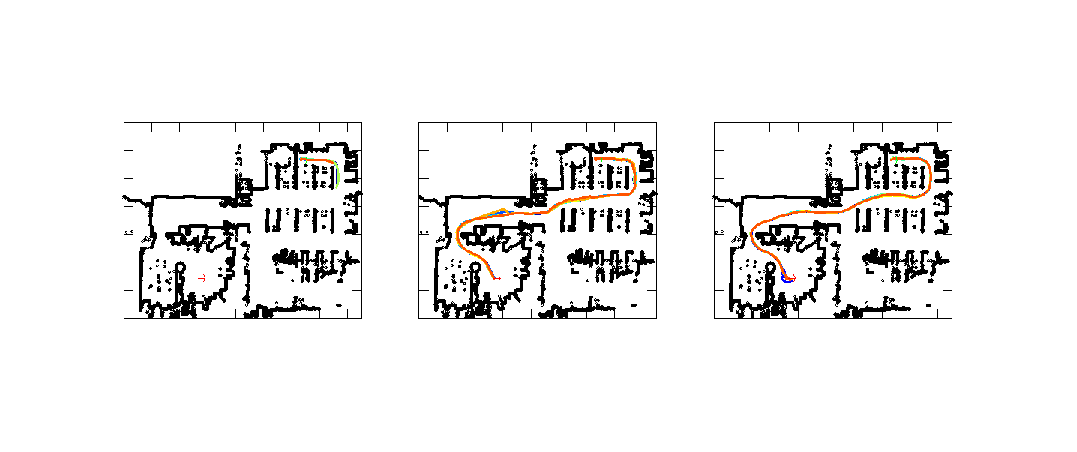
\includegraphics{./figures/parts/02/chapters/01/sections/04/pose_sbpl_csal}}%
    \gplfronttext
  \end{picture}%
\endgroup

  \end{subfigure}%
  \caption{\small Τα διανυθέντα μονοπάτια $\bm{\mathcal{P}}$ του ρομπότ, όπως
           ορίστηκαν από τους τρεις ελεγκτές κίνησης για κάθε συνδυασμό τους με
           αλγόριθμο παραγωγής μονοπατιών του πίνακα
           \ref{tbl:planners_sifted_list}, σε σχέση με τις ορισμένες αρχικές και
           τελικές στάσεις του περιβάλλοντος CSAL}
  \label{fig:poses:csal}
\end{figure*}

Ο πίνακας \ref{tbl:rank_csal} καταγράφει την τιμή-αξία $V_{\bm{M}_L}$
και την κατάταξη όλων των συνδυασμών αλγορίθμων χάραξης μονοπατιών και
ελεγκτών κίνησης που αξιολογήθηκαν με βάση τις τιμές όλων των μετρικών, που
παρουσιάζονται στους πίνακες
\ref{tbl:info_global_plan_csal}-\ref{tbl:info_deviation_from_global_plan_csal}
όσον αφορά στις επιδόσεις τους στην πλοήγηση στο περιβάλλον CSAL. Για τον
υπολογισμό της τιμής όλων των συνδυασμών, όλα τα βάρη $w_m = 1.0$ εκτός από
αυτό που αφορά στη μετρική $\mu_{PF} / \mu_{LPC}$, λόγω του γεγονότος ότι ότι ο
\texttt{eband\_local\_planner} δεν παρέχει πρόσβαση στον αριθμό των κλήσεων του
ελεγκτή. Λεπτομέρειες σχετικά με τις επιδόσεις των αλγορίθμων κατασκευής
μονοπατιών, των ελεγκτών κίνησης, και των συνδυασμών τους, βρίσκονται στο
παράρτημα \ref{appendix:evaluation_csal}.

Αυτό που ξεχωρίζει στα πειράματα στο πραγματικό περιβάλλον CSAL είναι ότι η
επίδοση των συνδυασμών του \texttt{sbpl\_lattice\_planner} με ελεγκτές κίνησης
μειώθηκε, επιτρέποντας στον \texttt{eband\_local\_planner} και τους συνδυασμούς
του να εκτοπίσουν τον συνδυασμό του \texttt{teb\_local\_planner} με τον
\texttt{sbpl\_lattice\_planner} από τις πρώτες θέσεις. Εκτός από αυτήν την
αλλαγή, οι συνδυασμοί των υπόλοιπων αλγορίθμων παρουσιάζουν το ίδιο μοτίβο που
παρατηρήθηκε στις προσομοιώσεις: (α) δεδομένου ενός αλγορίθμου κατασκευής
μονοπατιών, ο \texttt{teb\_local\_planner} υπερτερεί του
\texttt{eband\_local\_planner}, ο οποίος με τη σειρά του υπερτερεί του
\texttt{dwa\_local\_planner}, και (β) δεδομένου ενός ελεγκτή κίνησης, ο
\texttt{navfn} υπερτερεί του \texttt{global\_planner}.


\begin{table}[htb]\centering
\renewcommand{\arraystretch}{1.3}
\begin{tabular}{llccc}
  GP                     & LP             & επιτυχημένες αποστολές / $N$ & $V_{\bm{M}_C}$ & Κατάταξη \\ \toprule
  \texttt{navfn}         & \texttt{teb}   & $10/10$                      & $18.74$        & $1$      \\
  \texttt{globalplanner} & \texttt{teb}   & $10/10$                      & $16.84$        & $2$      \\
  \texttt{navfn}         & \texttt{eband} & $10/10$                      & $14.77$        & $3$      \\
  \texttt{globalplanner} & \texttt{eband} & $10/10$                      & $14.26$        & $4$      \\
  \texttt{sbpl}          & \texttt{teb}   & $10/10$                      & $13.57$        & $5$      \\
  \texttt{navfn}         & \texttt{dwa}   & $0/10$                       & $8.10$         & $6$      \\
  \texttt{sbpl}          & \texttt{eband} & $10/10$                      & $7.80$         & $7$      \\
  \texttt{sbpl}          & \texttt{dwa}   & $0/10$                       & $6.47$         & $8$      \\
  \texttt{globalplanner} & \texttt{dwa}   & $0/10$                       & $6.13$         & $9$      \\ \bottomrule
\end{tabular}
\caption{\small Οι αριθμοί επιτυχίας αποστολών, η τιμή-αξία $V_{\bm{M}_L}$, και
         η κατάταξη όλων των συνδυασμών των αλγορίθμων χάραξης μονοπατιών και
         ελεγκτών κίνησης που αξιολογούνται για τους την επίδοσή τους στο
         περιβάλλον CSAL σε $N=10$ πειράματα}
\label{tbl:rank_csal}
\end{table}


%%%%%%%%%%%%%%%%%%%%%%%%%%%%%%%%%%%%%%%%%%%%%%%%%%%%%%%%%%%%%%%%%%%%%%%%%%%%%%%%
\subsection{Συνολική αξιολόγηση}
  \label{subsection:02_01_04:05}

Ο πίνακας \ref{tbl:rank_overall} καταγράφει τις τελικές συνδυαστικές τιμές-αξίες
όλων των συνδυασμών των αλγορίθμων χάραξης μονοπατιών της αριστερής στήλης
του πίνακα \ref{tbl:planners_sifted_list} με όλους τους ελεγκτές κίνησης της
δεξιάς στήλης του ίδιου πίνακα, για όλα τα πειράματα και προσομοιώσεις που
διεξήχθησαν.

\begin{table}\centering
\renewcommand{\arraystretch}{1.3}
\begin{tabular}{llccccc}
  GP                      & LP              & $V_{\bm{M}_C}$ & $V_{\bm{M}_W}$ & $V_{\bm{M}_L}$ & $V$      & Κατάταξη \\ \toprule
  \texttt{navfn}          & \texttt{teb}    & $21.41$        & $20.00$        & $18.74$        & $60.15$  & $1$      \\
  \texttt{globalplanner}  & \texttt{teb}    & $19.29$        & $21.90$        & $16.84$        & $58.03$  & $2$      \\
  \texttt{sbpl}           & \texttt{teb}    & $20.35$        & $12.27$        & $13.57$        & $46.19$  & $3$      \\
  \texttt{navfn}          & \texttt{eband}  & $15.96$        & $11.76$        & $14.77$        & $42.49$  & $4$      \\
  \texttt{globalplanner}  & \texttt{eband}  & $14.70$        & $11.95$        & $14.26$        & $40.91$  & $5$      \\
  \texttt{sbpl}           & \texttt{eband}  & $10.99$        & $9.85$         & $7.80$         & $28.94$  & $6$      \\
  \texttt{navfn}          & \texttt{dwa}    & $6.46$         & $9.31$         & $8.10$         & $28.64$  & $7$      \\
  \texttt{globalplanner}  & \texttt{dwa}    & $5.50$         & $8.86$         & $6.13$         & $20.49$  & $8$      \\
  \texttt{sbpl}           & \texttt{dwa}    & $6.56$         & $4.85$         & $6.47$         & $17.88$  & $9$      \\ \bottomrule
\end{tabular}
\caption{\small Η σύνθετη τελική τιμή $V$ και η κατάταξη όλων των συνδυασμών
         αλγορίθμων χάραξης μονοπατιών και ελεγκτών κίνησης του πίνακα
         \ref{tbl:planners_sifted_list} ως αποτέλεσμα της αξιολόγησης της
         επίδοσής τους βάσει των μετρικών των πινάκων
         \ref{tbl:metrics_and_proportionality_global_planners},
         \ref{tbl:metrics_and_proportionality_local_planners}, και
         \ref{tbl:metrics_and_proportionality_combination_planners}, σε
         επαναληπτικές προσομοιώσεις και πειράματα στα περιβάλλοντα CORRIDOR
         (σχήμα \ref{fig:02_01_03:map_corridor}), WILLOWGARAGE (σχήμα
         \ref{fig:02_01_03:map_willowgarage}) και CSAL (σχήμα
         \ref{fig:02_01_03:map_csal})}
\label{tbl:rank_overall}
\end{table}

Με βάση τα παραπάνω στοιχεία δύο καθοριστικά πρότυπα αναδύονται με σαφήνεια:
Όσον αφορά στους ελεγκτές κίνησης: ο \texttt{teb\_local\_planner} υπερτερεί του
\texttt{eband\_local\_planner}, ο οποίος υπερτερεί με τη σειρά του του
\texttt{dwa\_local\_planner}. Όσον αφορά στους αλγορίθμους σχεδιασμού
μονοπατιών: δεδομένου ενός ελεγκτή κίνησης, ο \texttt{navfn} υπερτερεί του
\texttt{global\_planner} με μικρή διαφορά, μικρότερη από εκείνη μεταξύ του
τελευταίου και του \texttt{sbpl\_lattice\_planner}.

\begin{bw_box}
Με βάση τα πειραματικά δεδομένα (ενότητα \ref{subsection:02_01_03:01}
και παράρτημα \ref{appendix:01}), τις μετρικές αξιολόγησης τους (ενότητα
\ref{subsection:02_01_03:02}), τη μεθοδολογία αξιολόγησης (ενότητα
\ref{subsection:02_01_03:03}) και τις ποιοτικές μετρικές αξιολόγησης πακέτων
λογισμικού ROS (ενότητα \ref{subsection:02_01_03:04}), συμπεραίνουμε ότι ο
πιό αποτελεσματικός συνδυασμός πακέτων για χρήση στην αυτόνομη πλοήγηση στο
πεδίο εφαρμογής \ref{scope} χρησιμοποιεί τον \texttt{navfn} ως αλγόριθμο χάραξης
μονοπατιών (ενότητα \ref{subsubsection:02_01_02:03_01}), και τον
\texttt{teb\_local\_planner} ως ελεγκτή κίνησης (ενότητα
\ref{subsubsection:02_01_02:03_02}).
\end{bw_box}

Επιπλέον, οι καλύτεροι υποψήφιοι για την αντικατάσταση των παραπάνω
αλγορίθμων, ανάλογα με τις συνθήκες του περιβάλλοντος και τις
απαιτήσεις/στόχους πλοηγήσεις, είναι ο \texttt{global\_planner} και ο
\texttt{eband\_local\_planner} αντίστοιχα.
